% \iffalse meta-comment
%
% Copyright (C) 2014, 2015 by Thomas Weise <http://www.it-weise.de>
%
% This file may be distributed and/or modified under the conditions of
% the LaTeX Project Public License, either version 1.3 of this license
% or (at your option) any later version. The latest version of this
% license is in:
% 
%    http://www.latex-project.org/lppl.txt
% 
% \fi
%
% \iffalse
%<*driver>
\ProvidesFile{figureSeries.dtx}
%</driver>
%<package>\NeedsTeXFormat{LaTeX2e}[1999/12/01]
%<package>\ProvidesPackage{figureSeries}
%<*package>
    [2015/02/13 v0.9.4 Provides a floating, figure*-like construct that can break over multiple pages]
%</package>
%
%<*driver>
\documentclass{ltxdoc}
\usepackage{figureSeries}[2014/06/17]
\usepackage[%
breaklinks=true,%
colorlinks=true,%
urlcolor=black,%
menucolor=black,%
linkcolor=black,%
bookmarks=true,%
bookmarksopen=false,%
hyperfootnotes=true,%
citecolor=black,%
filecolor=black,%
pdfkeywords={LaTeX, package, figureSeries}
]{hyperref}%
\usepackage{breakurl}%
\usepackage[square,numbers,comma,sort&compress]{natbib}%
%
\usepackage{float}%
\floatstyle{ruled}%
\newfloat{example}{thp}{lop}%
\floatname{example}{Example}%
\usepackage{verbatim}%
%
%
\usepackage{graphicx}%
\usepackage{subcaption}%
%
\EnableCrossrefs         
\CodelineIndex
\RecordChanges
%
%
\begin{document}
  \DocInput{figureSeries.dtx}
  \PrintChanges
  \PrintIndex
\end{document}
%</driver>
% \fi
%
% \CheckSum{215}
%
% \CharacterTable
%  {Upper-case    \A\B\C\D\E\F\G\H\I\J\K\L\M\N\O\P\Q\R\S\T\U\V\W\X\Y\Z
%   Lower-case    \a\b\c\d\e\f\g\h\i\j\k\l\m\n\o\p\q\r\s\t\u\v\w\x\y\z
%   Digits        \0\1\2\3\4\5\6\7\8\9
%   Exclamation   \!     Double quote  \"     Hash (number) \#
%   Dollar        \$     Percent       \%     Ampersand     \&
%   Acute accent  \'     Left paren    \(     Right paren   \)
%   Asterisk      \*     Plus          \+     Comma         \,
%   Minus         \-     Point         \.     Solidus       \/
%   Colon         \:     Semicolon     \;     Less than     \<
%   Equals        \=     Greater than  \>     Question mark \?
%   Commercial at \@     Left bracket  \[     Backslash     \\
%   Right bracket \]     Circumflex    \^     Underscore    \_
%   Grave accent  \`     Left brace    \{     Vertical bar  \|
%   Right brace   \}     Tilde         \~}
%
%
% \changes{v0.9.0}{2014/06/17}{Initial Draft Version}
% \changes{v0.9.1}{2014/06/18}{Better examples showing the shortcomings of the package (in particular in two-column mode).}
% \changes{v0.9.2}{2015/02/13}{Shortcomings in two-column mode fixed: vertical column starts are now aligned well.}
% \changes{v0.9.3}{2015/07/07}{Failed attempt to fix ``Float(s) lost!'' errors.}
% \changes{v0.9.4}{2015/07/09}{To do.}
%
% \GetFileInfo{figureSeries.dtx}
%
% \DoNotIndex{\def,\if,\fi}
% 
%
% \title{The \textsf{figureSeries} package\thanks{This document
%   corresponds to \textsf{figureSeries}~\fileversion, dated \filedate.}}
% \author{Thomas Weise\\%
% \resizebox{0.95\textwidth}{!}{\parbox{1.5\textwidth}{\centering%
% {Nature Inspired Computation and Applications Laboratory}\\%
% {USTC-Birmingham Joint Research Institute in Intelligent Computation and Its Applications}\\%
% {School of Computer Science and Technology (SCST)}\\%
% {University of Science and Technology of China (USTC)}\\%
% {West Campus, Science and Technology Building, West Wing, Room 601}\\
% {Huangshan Road/Feixi Road, Hefei 230027, Anhui, China}\\%
% {\texttt{tweise@ustc.edu.cn} $\cdot$ \texttt{tweise@gmx.de}} $\cdot$ \texttt{http://www.it-weise.de/}\\%
% }}}%
% \date{\filedate}
%
% \maketitle
%
% \begin{abstract}
% This package provides a first working version of a figure*-like construct, which
% can contain arbitrarily many sub-figures, (somewhat) float, and automatically break
% over multiple pages if necessary. The most current source code of this package
% can be found online at \url{http://github.com/thomasWeise/figureSeries}. Some
% discussions and additional information may be found at \url{http://www.it-weise.de}.
% \end{abstract}
%
% \setcounter{tocdepth}{2}
% \tableofcontents
%
% \section{Introduction}%
%
% \subsection{Addressed Problem and Use Case}%
% \LaTeX\ documents can contain floating objects such as figures
% or tables. ``floating'' here means that you insert a figure somewhere
% in your text and \LaTeX\ will find the best place where to put it for
% you, a place where it fits nicely into the overall layout of the
% document. Sometimes it is desirable that a figure contains several
% sub-figures. Let's say you want to group several diagrams which show
% related information and which all have the same structure.
%
% In \LaTeX, a floating object (composed of its contents and potentially
% a caption) can occupy at most one full page, meaning that it cannot
% contain any page break. This, in turn, means that the number of (or
% better the space for) sub-figures that can be hosted inside a figure
% is limited as well. But what if we have too many sub-figures? 
% What it the sub-figures do not fit on one page, into one
% floating object, into one |\begin{figure}...\end{figure}|? (Again: The
% required space includes the space for the sub-figures themselves, their
% captions, the vertical space between rows of sub-figures, and the caption
% of the hosting figure.)
%
% We can somewhat solve this issue by splitting the hosting figure
% into several separate figures, each containing a feasible amount of sub-figures.
% This needs to be done by hand, because we need to compile the document
% and fix and compile and fix and so on, since we usually not know beforehand
% how many sub-figures fit into one figure. This is not nice.
%
% Problems may occur when our \LaTeX\ document is created automatically and
% has an \emph{a priori} unknown number of sub-figures in a figure. There is
% no way to automatically determine how many sub-figures we can place into a
% figure. Even if we would know the sub-figure sizes, we cannot compute the
% space occupied by their captions beforehand (well, without replicating \LaTeX, that is\dots).
% Trust me, I have tried this (in the software project \emph{TSPSuite}~\cite{WCTLTCMY2014BOAAOSFFTTSP}).
% Similar use cases have been reported in~\cite{K2009SOAFOMP,AV2011SSAMPBP}.
%
% Also, \LaTeX\ is limited in terms of the number of floating objects
% it can handle, I believe the limit is 18 and can be increased
% using the package |morefloats|~\cite{MH2012TMP}, but this is a true problem when creating
% many sub-figures automatically. You may have so many sub-figures that
% splitting them into multiple (hosting) figures leads to too many (hosting) 
% figures. Or you just end up with too many floating objects which are all
% laid out at once at the end of a chapter or something or which otherwise make
% your text layout look odd and unbalanced.
%
% \subsection{Provided Functionality}%
% This package provides%
% \begin{enumerate}%
% \item a facility to include an arbitrary number of (potentially differently-sized) sub-figures into a figure*-like construct,%
% \item the ability to make this figure*-like construct look as if it was a floating object, which%
% \item works well in both single-column and double-column documents.%
% \end{enumerate}%
%
% \textbf{WARNING:}~This is just a  first, hacked-together version
% of this package. I am not an expert in \LaTeX, and I am pretty sure
% I managed to incorporate a few ``that cannot be made to work reliable''s
% into the code. Plus, it contains some code taken from the internet, which
% I myself only partially understand (see Section~\ref{sec:codeBasedOnLong2}).
% This package here is just there for discussion. Use it at your own risk.%
%
% \section{Usage}%
%
% \subsection{Loading the Package}
% Load this package using
% \begin{quote}
%   |\RequirePackage{figureSeries}|
% \end{quote}
% This will automatically load the packages |caption|~\cite{S2011TCPCCIFE}, |subcaption|~\cite{S2013TSPSFSC}, and |afterpage|~\cite{C1995TAPECATPB}.
%
% \subsection{Provided Macros}\label{sec:providedMacros}%
%
% Here we discuss the macros that can directly be accessed by the user to make use of the package's
% functionality. The implementation of these macros is given in Section~\ref{sec:userInterfaceMacros}
% and several examples can be found in Section~\ref{sec:examples}.
%
% \DescribeMacro{\figureSeriesElement}
% The  macro |\figureSeriesElement|\marg{caption}\marg{contents} inserts an element of the figure series, i.e., one sub-figure.
% Its first argument is the caption of the element and may contain a |\label|.
% The second argument is the graphic to print. It could, e.g., be a call to |\includegraphic|
% from the |graphicx| package~\cite{CR2014PITGB}.
%
% \DescribeMacro{\figureSeriesRow}
% |\figureSeriesElement|\marg{contents} inserts a new row of elements (sub-figures) into
% the figure series. Its single argument should thus contain a sequence of |\figureSeriesElement|s.
% As a consequence of this architecture, each sub-figure belongs to one row and no sub-figure can
% span multiple rows.
%
% \DescribeMacro{\figureSeriesHere}
% The  macro |\figureSeriesHere|\marg{caption}\marg{contents} tries to insert a (non-floating) figure
% series at the current position in the document. This means that it may begin wherever, well, it
% is used, e.g., in the middle of the page.
%
% The macro has two mandatory parameters, the caption and the contents. The caption will be
% be put at the beginning of the figure series, which is different from the normal behavior of
% captions in |\begin{figure*}...\end{figure*}| or |\begin{figure}...\end{figure}|. The reason
% is that a figure series may span over multiple pages and having the caption at the end may
% be awkward and confusing. The caption text may contain a |\label|.
%
% The contents of a figure series should be a sequence of |\figureSeriesRow| calls.
%
% Since figure series are page-wide elements, starting them in the middle of the page only works
% in single-column documents. In two-column documents, any figure series will behave as specified in
% macro |\figureSeriesFloat| below.
%
% \DescribeMacro{\figureSeriesFloat}
% The  macro |\figureSeriesFloat|\marg{caption}\marg{contents} macro takes the same parameters
% as |\figureSeriesHere|, but has a float-like behavior. By using the |\afterpage| command of
% |afterpage| package~\cite{C1995TAPECATPB}, we let it start at the following page. This is different from \LaTeX'
% normal floating behavior, but as good as we can get with page-breaking objects, I think.
%
% \subsection{Examples}\label{sec:examples}%
%
% Here we provide a set of examples for the use of the package. Each example demonstrates another
% facet of the package and, at the same time, serves as test case. Instead of using |\includegraphic|,
% we simply stretch single letters via |\resizebox| and use them ``sub-figures''. This is good enough
% to see how the layout works and allows us to generate arbitrarily-sized placeholders for figures.
%
% In order to create some placeholder text in the examples, we use the |lipsum| command from package
% |lipsum|~\cite{H2914LAT1POLIDT}, which prints pseudo-Latin text known
% as ``Lorem Ipsum'' (see \url{http://en.wikipedia.org/wiki/Lorem_ipsum}).
%
% \subsubsection{Non-Floating Figure Series in Single-Column Document}%
% In Example~\ref{ex:llncs} we place a non-floating figure series consisting of two rows of
% figures into a single-column document using Springer's document class |llncs|~\cite{SPRINGERLNCS}.
% The result can be seen in Figure~\ref{ex:llncs:res} and compared with a floating version in Figure~\ref{ex:llncs2:res},
% which represents the floating version of this example (given in Example~\ref{ex:llncs2}).
% 
% \begin{example}%
% \begin{small}\verbatiminput{examples/example_1_LNCS.tex}\end{small}%
% \caption{An example using the single-column \texttt{llncs} class, rendered as Figure~\ref{ex:llncs:res}.}%
% \label{ex:llncs}%
% \end{example}%
%
% \begin{figure}%
% \begin{center}%
% \strut\hfill\strut%
% \subcaptionbox{Page 1 of the pdf compiled from Example~\ref{ex:llncs}.
% }{%
% \fbox{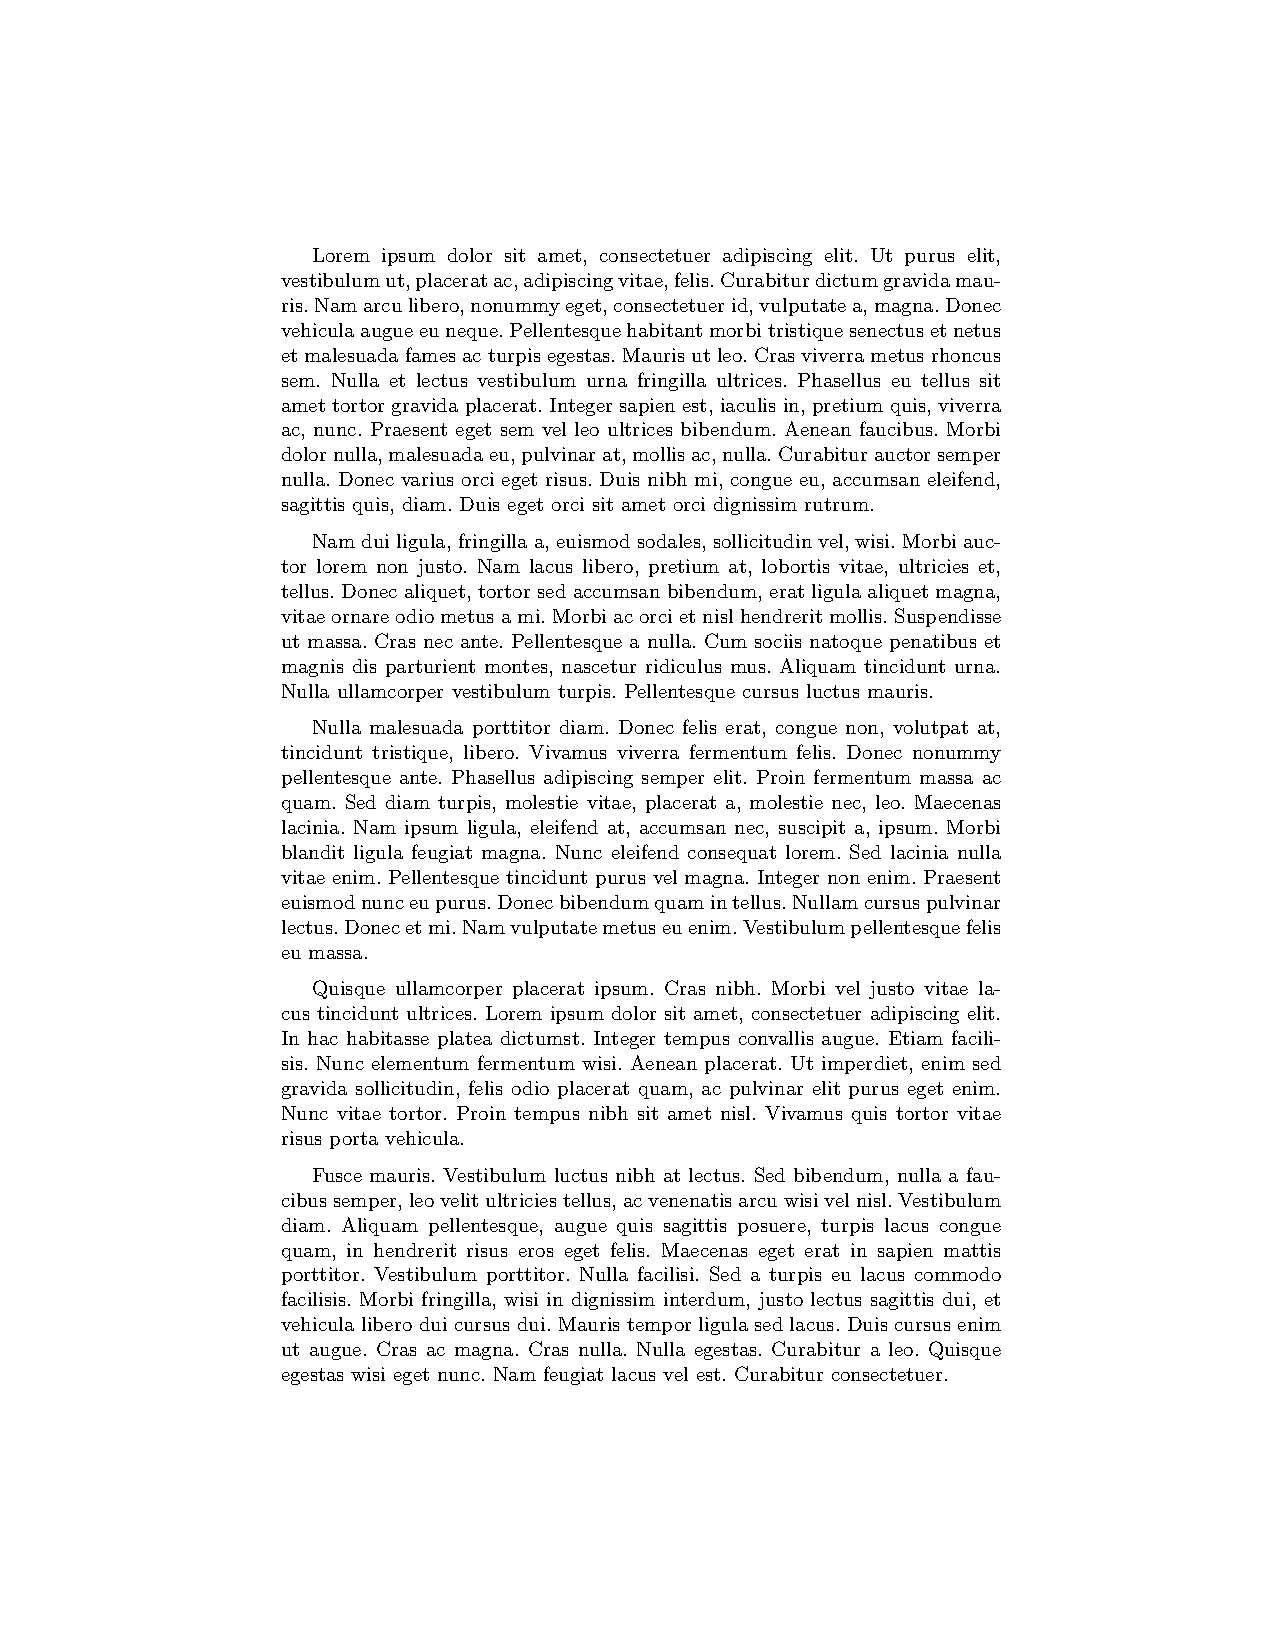
\includegraphics[page=1,width=0.412225\textwidth,trim=1.75in 1.65in 1.75in 1.5in,clip]{examples/example_1_LNCS.pdf}}%
% }%
% \strut\hfill\strut\hfill\strut%
% \subcaptionbox{Page 2 of the pdf compiled from Example~\ref{ex:llncs}.
% }{%
% \fbox{\includegraphics[page=2,width=0.412225\textwidth,trim=1.75in 1.65in 1.75in 1.5in,clip]{examples/example_1_LNCS.pdf}}%
% }%
% \strut\hfill\strut%
% \\%
% \strut\hfill\strut%
% \subcaptionbox{Page 3 of the pdf compiled from Example~\ref{ex:llncs}.
% }{%
% \fbox{\includegraphics[page=3,width=0.412225\textwidth,trim=1.75in 1.65in 1.75in 1.5in,clip]{examples/example_1_LNCS.pdf}}%
% }%
% \strut\hfill\strut\hfill\strut%
% \subcaptionbox{Page 4 of the pdf compiled from Example~\ref{ex:llncs}.
% }{%
% \fbox{\includegraphics[page=4,width=0.412225\textwidth,trim=1.75in 1.65in 1.75in 1.5in,clip]{examples/example_1_LNCS.pdf}}%
% }%
% \strut\hfill\strut%
% \caption{The rendered result of Example~\ref{ex:llncs} (with trimmed page margins): %
% A \texttt{figureSeries} starts at the bottom of a page and extends to the top of the next page.}%
% \label{ex:llncs:res}%
% \end{center}%
% \end{figure}%
% 
% \afterpage{\clearpage}%
%
% \subsubsection{Floating Figure Series in Double-Column Document}
% We now put a floating figure series into a double-column document using the
% |IEEEtran|~\cite{IEEETRAN} class in Example~\ref{ex:ieeetran1}.
% This new figure series has five rows of sub-figures and
% should span over multiple pages. The two-column text continues directly
% after the figure series. The rendered results of this example are given
% in Figure~\ref{ex:ieeetran1:res}.
%
% \begin{example}%
% \begin{small}\verbatiminput{examples/example_2_IEEEtran.tex}\end{small}%
% \caption{An example using the double-column \texttt{IEEEtrans} class, rendered as Figure~\ref{ex:ieeetran1:res}.}%
% \label{ex:ieeetran1}%
% \end{example}%
%
% \begin{figure}%
% \begin{center}%
% \strut\hfill\strut%
% \subcaptionbox{Page 1 of the pdf compiled from Example~\ref{ex:ieeetran1}.
% }{%
% \fbox{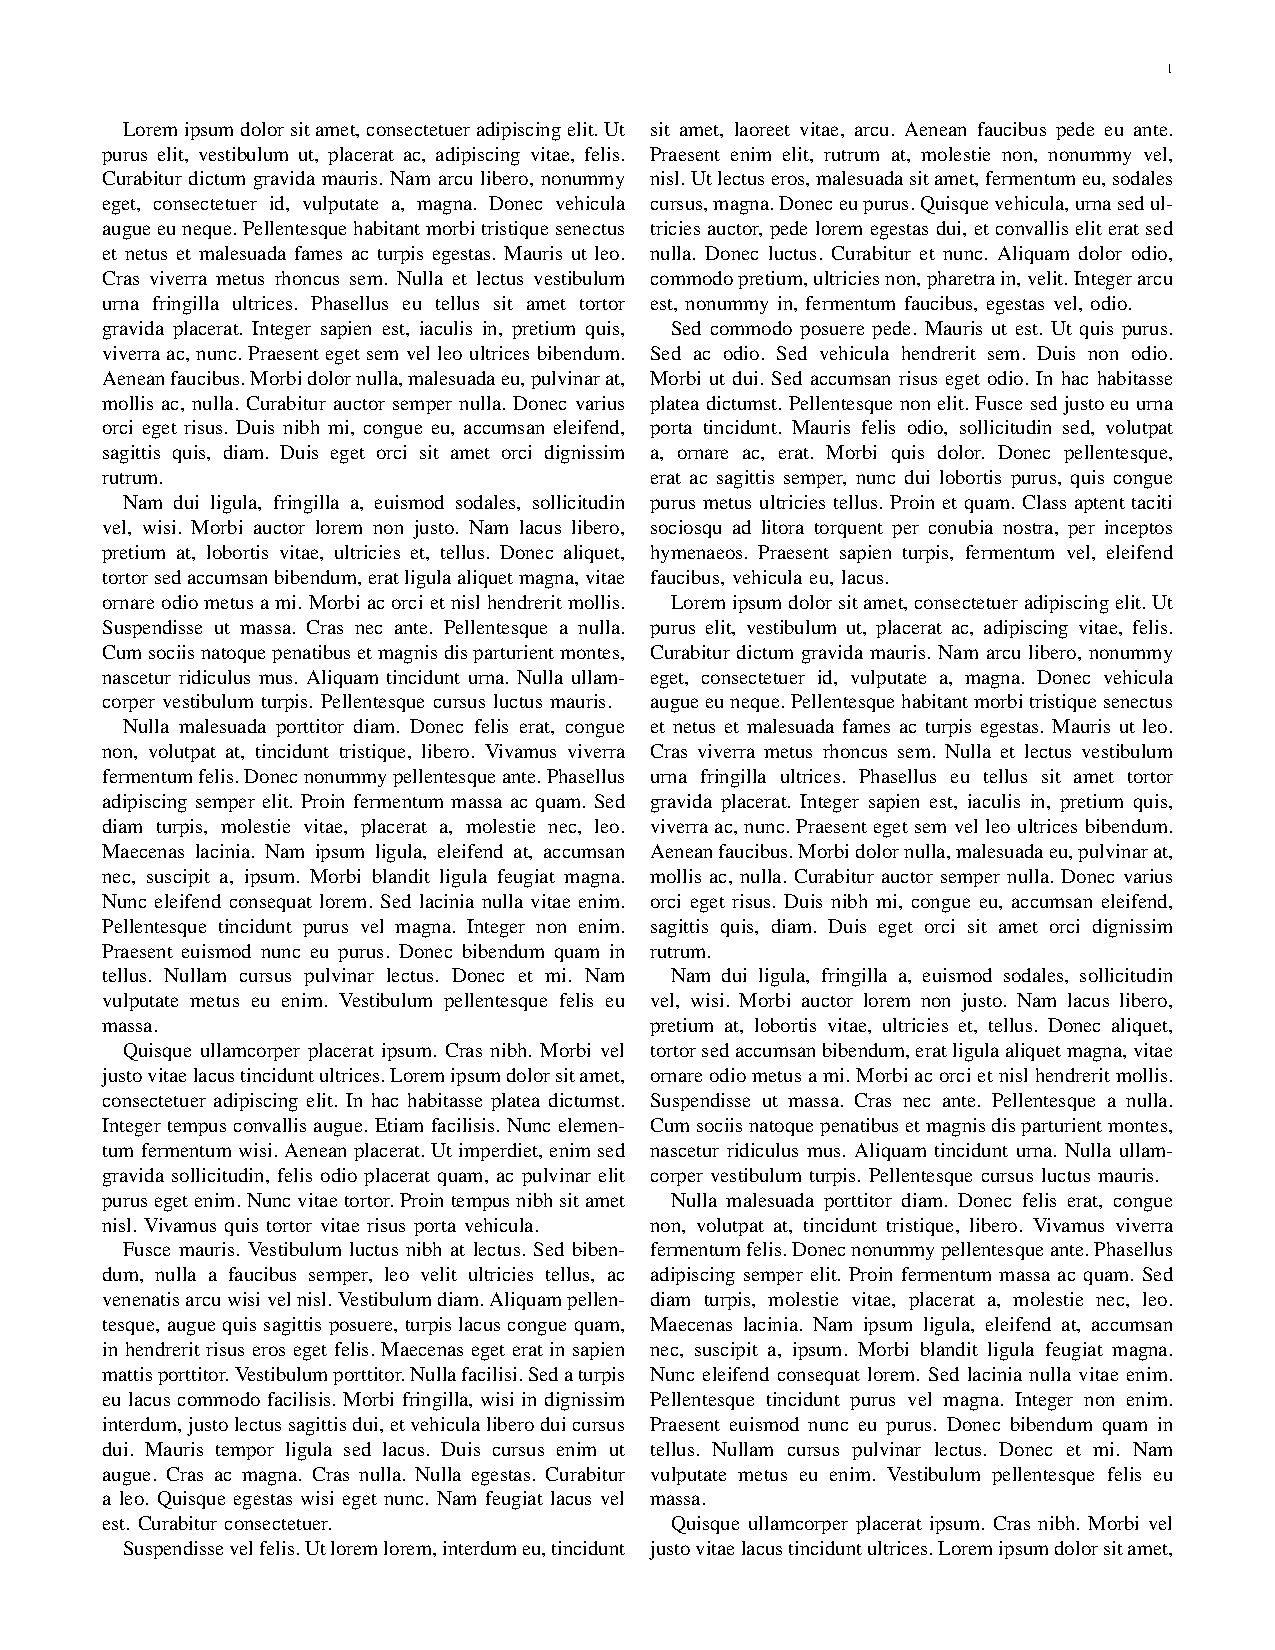
\includegraphics[page=1,width=0.45\textwidth,trim=0.65in 0.35in 0.65in 0.75in,clip]{examples/example_2_IEEEtran.pdf}}%
% }%
% \strut\hfill\strut\hfill\strut%
% \subcaptionbox{Page 2 of the pdf compiled from Example~\ref{ex:ieeetran1}.
% }{%
% \fbox{\includegraphics[page=2,width=0.45\textwidth,trim=0.65in 0.35in 0.65in 0.75in,clip]{examples/example_2_IEEEtran.pdf}}%
% }%
% \strut\hfill\strut%
% \\%
% \strut\hfill\strut%
% \subcaptionbox{Page 3 of the pdf compiled from Example~\ref{ex:ieeetran1}.
% }{%
% \fbox{\includegraphics[page=3,width=0.45\textwidth,trim=0.65in 0.35in 0.65in 0.75in,clip]{examples/example_2_IEEEtran.pdf}}%
% }%
% \strut\hfill\strut\hfill\strut%
% \subcaptionbox{Page 4 of the pdf compiled from Example~\ref{ex:ieeetran1}.
% }{%
% \fbox{\includegraphics[page=4,width=0.45\textwidth,trim=0.65in 0.35in 0.65in 0.75in,clip]{examples/example_2_IEEEtran.pdf}}%
% }%
% \strut\hfill\strut%
% \caption{The rendered result of Example~\ref{ex:ieeetran1} (with trimmed page margins): %
% A floating \texttt{figureSeries} in double-column mode.}%
% \label{ex:ieeetran1:res}%
% \end{center}%
% \end{figure}%
%
% \afterpage{\clearpage}%
%
% \subsubsection{Coalescing Figure Series in Double-Column Document}
% In Example~\ref{ex:ieeetran2}, we put several floating figure series close to
% each other into a double-column document, again using the |IEEEtran| class~\cite{IEEETRAN}.
% The bodies of the figure series should coalesce without losing their captions, figure
% numbers, or identities. Since they coalesce, no empty pages are produced in between (see \mbox{Section~\ref{sec:extendBody}.F}).
% The result is rendered as Figure~\ref{ex:ieeetran2:res}.
%
% \begin{example}%
% \begin{small}\verbatiminput{examples/example_3_IEEEtran.tex}\end{small}%
% \caption{An example using the double-column \texttt{IEEEtrans} class and two 
% coalescing figure series, rendered as Figure~\ref{ex:ieeetran2:res}.}%
% \label{ex:ieeetran2}%
% \end{example}%
%
% \begin{figure}%
% \begin{center}%
% \strut\hfill\strut%
% \subcaptionbox{Page 1 of the pdf compiled from Example~\ref{ex:ieeetran2}.
% }{%
% \fbox{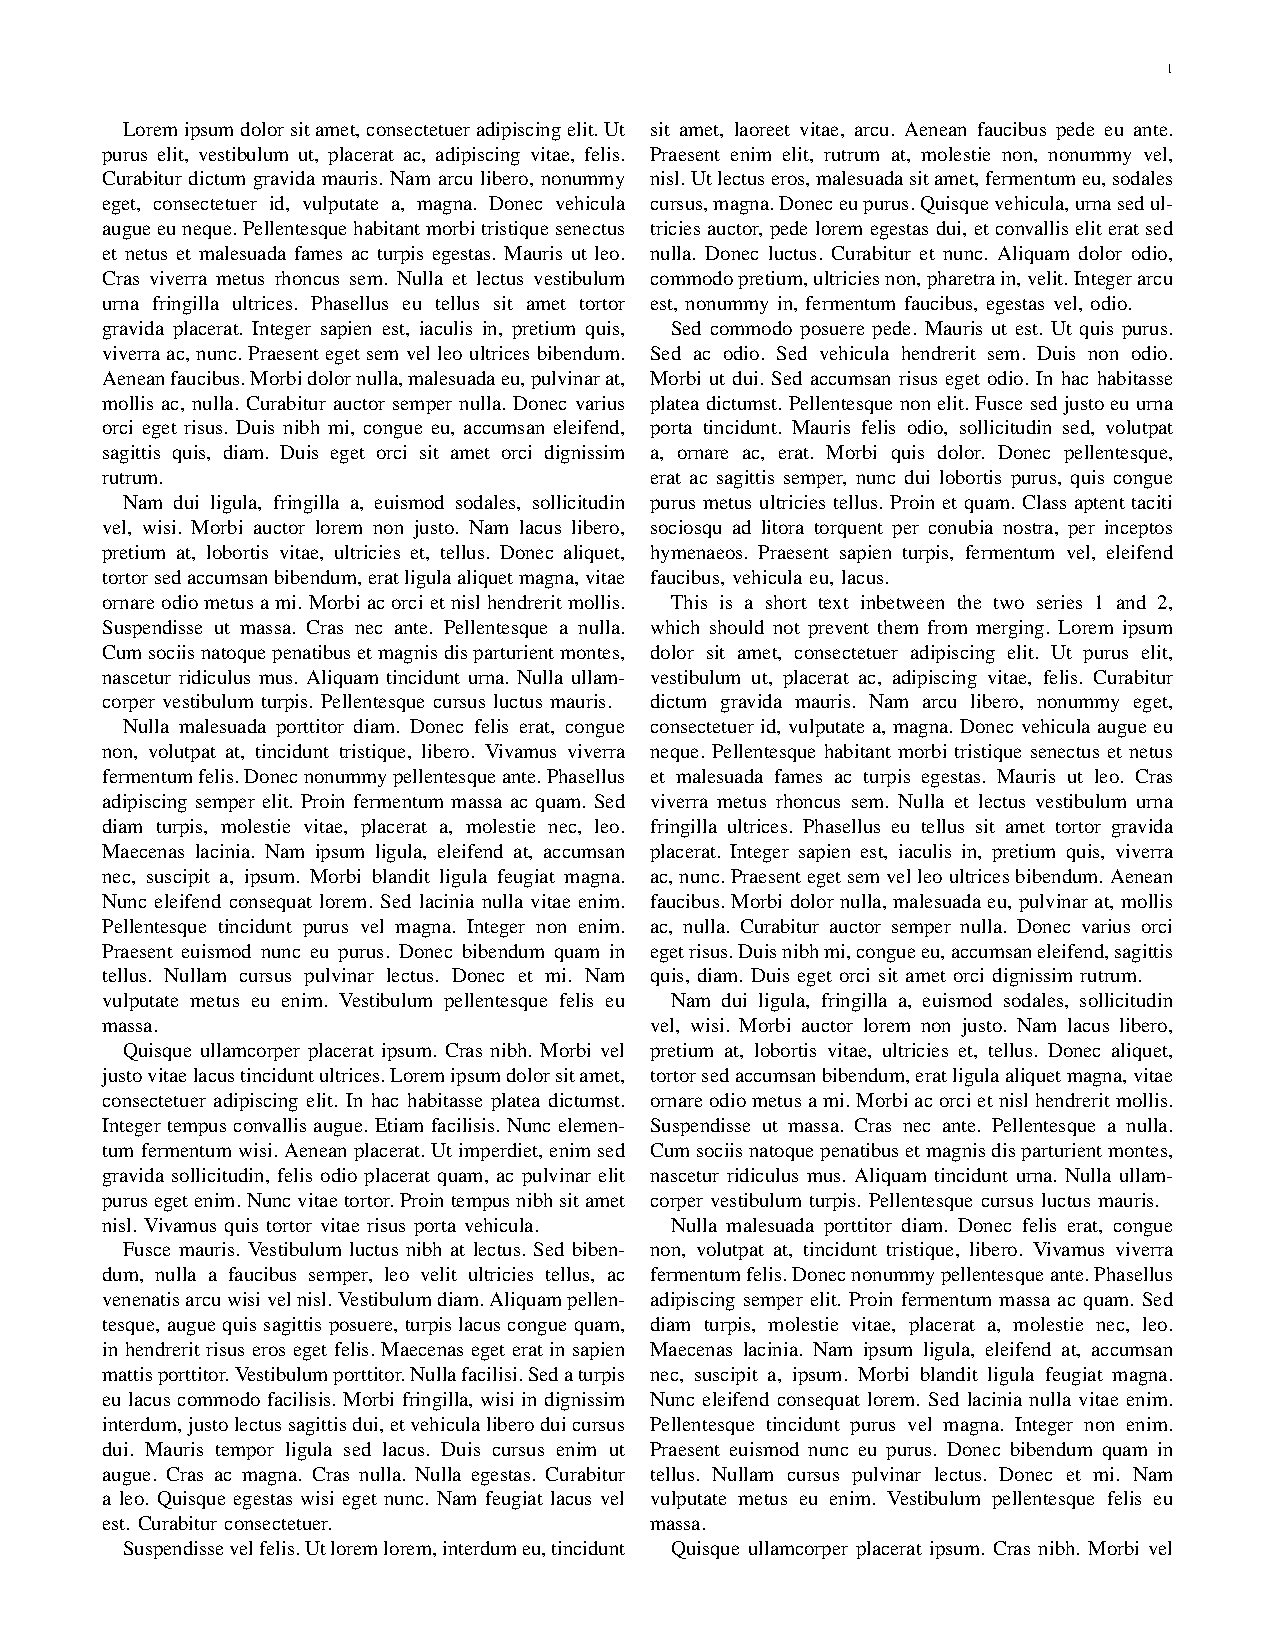
\includegraphics[page=1,width=0.45\textwidth,trim=0.65in 0.35in 0.65in 0.75in,clip]{examples/example_3_IEEEtran.pdf}}%
% }%
% \strut\hfill\strut\hfill\strut%
% \subcaptionbox{Page 2 of the pdf compiled from Example~\ref{ex:ieeetran2}.
% }{%
% \fbox{\includegraphics[page=2,width=0.45\textwidth,trim=0.65in 0.35in 0.65in 0.75in,clip]{examples/example_3_IEEEtran.pdf}}%
% }%
% \strut\hfill\strut%
% \\%
% \strut\hfill\strut%
% \subcaptionbox{Page 3 of the pdf compiled from Example~\ref{ex:ieeetran2}.
% }{%
% \fbox{\includegraphics[page=3,width=0.45\textwidth,trim=0.65in 0.35in 0.65in 0.75in,clip]{examples/example_3_IEEEtran.pdf}}%
% }%
% \strut\hfill\strut\hfill\strut%
% \subcaptionbox{Page 4 of the pdf compiled from Example~\ref{ex:ieeetran2}.
% }{%
% \fbox{\includegraphics[page=4,width=0.45\textwidth,trim=0.65in 0.35in 0.65in 0.75in,clip]{examples/example_3_IEEEtran.pdf}}%
% }%
% \strut\hfill\strut%
% \caption{The rendered result of Example~\ref{ex:ieeetran2} (with trimmed page margins): %
% Two floating \texttt{figureSeries} in double-column mode are coalesced, without using their caption and identies.}%
% \label{ex:ieeetran2:res}%
% \end{center}%
% \end{figure}%
%
% {\clearpage}%
% 
% \subsubsection{Double-Column Document with \texttt{sig-alternate}}
% In the following Example~\ref{ex:acm}, we test the |figureSeries| together for documents
% using ACM's |sig-alternate|~\cite{ACMSIGALTERNATE} document class.
%
% \begin{example}%
% \begin{small}\verbatiminput{examples/example_4_sigAlternate.tex}\end{small}%
% \caption{An example featuring the double-column \texttt{sig-alternate} class. %
% The results are rendered as Figure~\ref{ex:acm:res}.}%
% \label{ex:acm}%
% \end{example}%
%
% \begin{figure}%
% \begin{center}%
% \strut\hfill\strut%
% \subcaptionbox{Page 1 of the pdf compiled from Example~\ref{ex:acm}.
% }{%
% \fbox{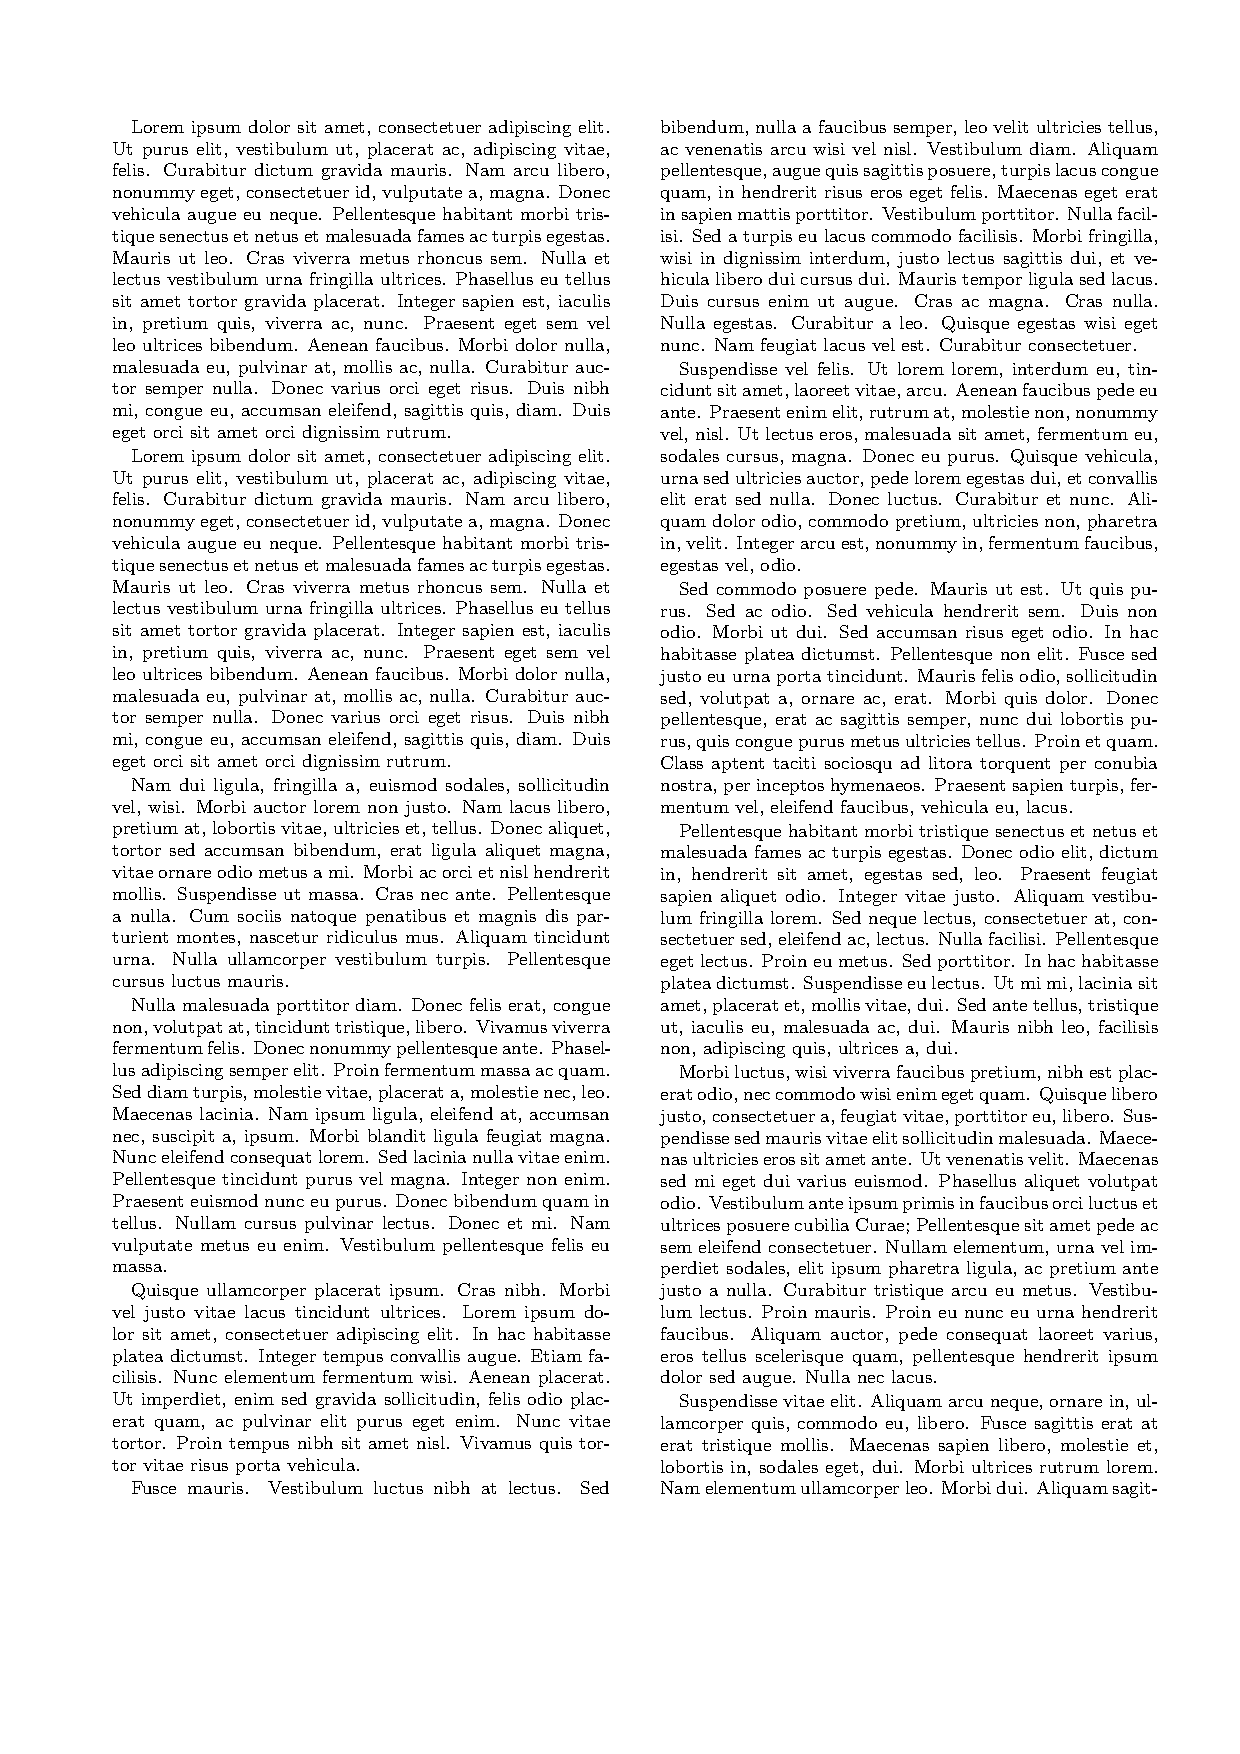
\includegraphics[page=1,width=0.45\textwidth,trim=0.5in 0.5in 0.5in 0.5in,clip]{examples/example_4_sigAlternate.pdf}}%
% }%
% \strut\hfill\strut\hfill\strut%
% \subcaptionbox{Page 2 of the pdf compiled from Example~\ref{ex:acm}.
% }{%
% \fbox{\includegraphics[page=2,width=0.45\textwidth,trim=0.5in 0.5in 0.5in 0.5in,clip]{examples/example_4_sigAlternate.pdf}}%
% }%
% \strut\hfill\strut%
% \\%
% \strut\hfill\strut%
% \subcaptionbox{Page 3 of the pdf compiled from Example~\ref{ex:acm}.
% }{%
% \fbox{\includegraphics[page=3,width=0.45\textwidth,trim=0.5in 0.5in 0.5in 0.5in,clip]{examples/example_4_sigAlternate.pdf}}%
% }%
% \strut\hfill\strut\hfill\strut%
% \subcaptionbox{Page 4 of the pdf compiled from Example~\ref{ex:acm}.
% }{%
% \fbox{\includegraphics[page=4,width=0.45\textwidth,trim=0.5in 0.5in 0.5in 0.5in,clip]{examples/example_4_sigAlternate.pdf}}%
% }%
% \strut\hfill\strut%
% \caption{The rendered result of Example~\ref{ex:acm} (with trimmed page margins): %
% It works for \texttt{sig-alternate} too.}%
% \label{ex:acm:res}%
% \end{center}%
% \end{figure}%
%
%
% \afterpage{\clearpage}%
% 
% \subsubsection{Many Small Sub-Figures in Double-Column Document}
% In the following Example~\ref{ex:acm2} (again based on ACM's |sig-alternate|~\cite{ACMSIGALTERNATE}
% document class), we put many small sub-figures into a figure. Also, the last paragraph of the text
% in the example is a reference to one of the sub-figures. The results are rendered as Figure~\ref{ex:acm2:res}.
%
% \begin{example}%
% \begin{small}\verbatiminput{examples/example_5_sigAlternate.tex}\end{small}%
% \caption{An example featuring the double-column \texttt{sig-alternate} class with a reference to sub-figure. %
% The results are rendered as Figure~\ref{ex:acm2:res}.}%
% \label{ex:acm2}%
% \end{example}%
%
% \begin{figure}%
% \begin{center}%
% \strut\hfill\strut%
% \subcaptionbox{Page 1 of the pdf compiled from Example~\ref{ex:acm2}.
% }{%
% \fbox{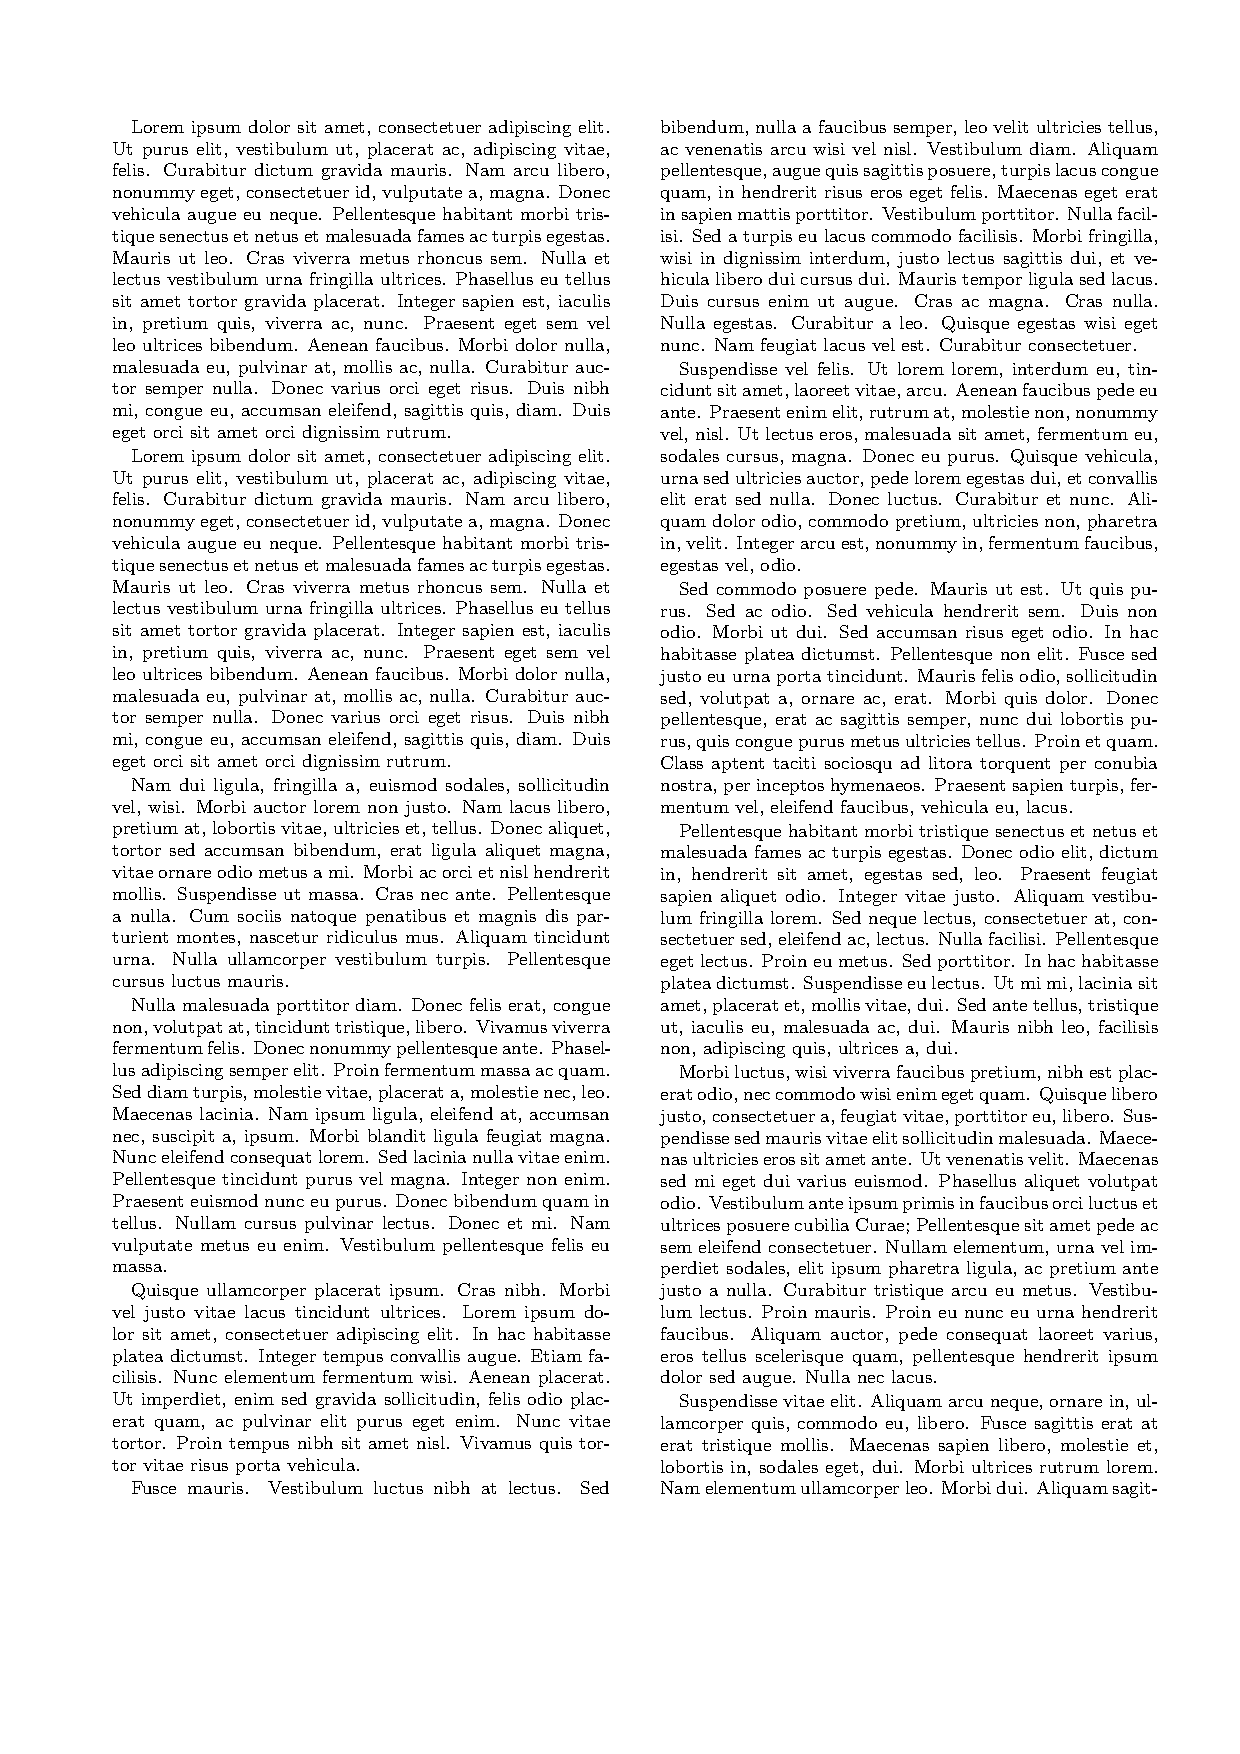
\includegraphics[page=1,width=0.45\textwidth,trim=0.5in 0.5in 0.5in 0.5in,clip]{examples/example_5_sigAlternate.pdf}}%
% }%
% \strut\hfill\strut\hfill\strut%
% \subcaptionbox{Page 2 of the pdf compiled from Example~\ref{ex:acm2}.
% }{%
% \fbox{\includegraphics[page=2,width=0.45\textwidth,trim=0.5in 0.5in 0.5in 0.5in,clip]{examples/example_5_sigAlternate.pdf}}%
% }%
% \strut\hfill\strut%
% \\%
% \strut\hfill\strut%
% \subcaptionbox{Page 3 of the pdf compiled from Example~\ref{ex:acm2}.
% }{%
% \fbox{\includegraphics[page=3,width=0.45\textwidth,trim=0.5in 0.5in 0.5in 0.5in,clip]{examples/example_5_sigAlternate.pdf}}%
% }%
% \strut\hfill\strut\hfill\strut%
% \subcaptionbox{Page 4 of the pdf compiled from Example~\ref{ex:acm2}.
% }{%
% \fbox{\includegraphics[page=4,width=0.45\textwidth,trim=0.5in 0.5in 0.5in 0.5in,clip]{examples/example_5_sigAlternate.pdf}}%
% }%
% \strut\hfill\strut%
% \caption{The rendered result of Example~\ref{ex:acm2} (with trimmed page margins): %
% Many small sub-figures nicely fill a page.}%
% \label{ex:acm2:res}%
% \end{center}%
% \end{figure}%
%
%
% \afterpage{\clearpage}%
% 
% \subsubsection{Two \texttt{figureSeries} Separated by Text in Double-Column Document}
% In the following Example~\ref{ex:acm3} (again based on ACM's |sig-alternate|~\cite{ACMSIGALTERNATE}
% document class), we put two |figureSeries| which are separated by text.
% The results are rendered as Figure~\ref{ex:acm3:res}.
%
% \begin{example}%
% \begin{small}\verbatiminput{examples/example_6_sigAlternate.tex}\end{small}%
% \caption{An example featuring two figure series separated by text. %
% The results are rendered as Figure~\ref{ex:acm3:res}.}%
% \label{ex:acm3}%
% \end{example}%
%
% \begin{figure}%
% \begin{center}%
% \strut\hfill\strut%
% \subcaptionbox{Page 2 of the pdf compiled from Example~\ref{ex:acm3}.
% }{%
% \fbox{\includegraphics[page=2,width=0.45\textwidth,trim=0.5in 0.5in 0.5in 0.5in,clip]{examples/example_6_sigAlternate.pdf}}%
% }%
% \strut\hfill\strut\hfill\strut%
% \subcaptionbox{Page 3 of the pdf compiled from Example~\ref{ex:acm3}.
% }{%
% \fbox{\includegraphics[page=3,width=0.45\textwidth,trim=0.5in 0.5in 0.5in 0.5in,clip]{examples/example_6_sigAlternate.pdf}}%
% }%
% \strut\hfill\strut%
% \\%
% \strut\hfill\strut%
% \subcaptionbox{Page 6 of the pdf compiled from Example~\ref{ex:acm3}.
% }{%
% \fbox{\includegraphics[page=6,width=0.45\textwidth,trim=0.5in 0.5in 0.5in 0.5in,clip]{examples/example_6_sigAlternate.pdf}}%
% }%
% \strut\hfill\strut\hfill\strut%
% \subcaptionbox{Page 8 of the pdf compiled from Example~\ref{ex:acm3}.
% }{%
% \fbox{\includegraphics[page=8,width=0.45\textwidth,trim=0.5in 0.5in 0.5in 0.5in,clip]{examples/example_6_sigAlternate.pdf}}%
% }%
% \strut\hfill\strut%
% \caption{The rendered result of Example~\ref{ex:acm3} (with trimmed page margins): %
% Two \texttt{figureSeries} are separated by text.}%
% \label{ex:acm3:res}%
% \end{center}%
% \end{figure}%
%
% \afterpage{\clearpage}%
%
% \subsubsection{One Floating \texttt{figureSeries} in a Single-Column Document}
% In the following Example~\ref{ex:llncs2} (based on Springer's |llncs|~\cite{SPRINGERLNCS}
% document class), we let the figure series from Example~\ref{ex:llncs} float.
% You can compare the rendered in Figure~\ref{ex:llncs2:res} with those in Figure~\ref{ex:llncs:res}.
%
% \begin{example}%
% \begin{small}\verbatiminput{examples/example_7_LNCS.tex}\end{small}%
% \caption{An example using the single-column \texttt{llncs} class, rendered as Figure~\ref{ex:llncs2:res}.}%
% \label{ex:llncs2}%
% \end{example}%
%
% \begin{figure}%
% \begin{center}%
% \strut\hfill\strut%
% \subcaptionbox{Page 1 of the pdf compiled from Example~\ref{ex:llncs2}.
% }{%
% \fbox{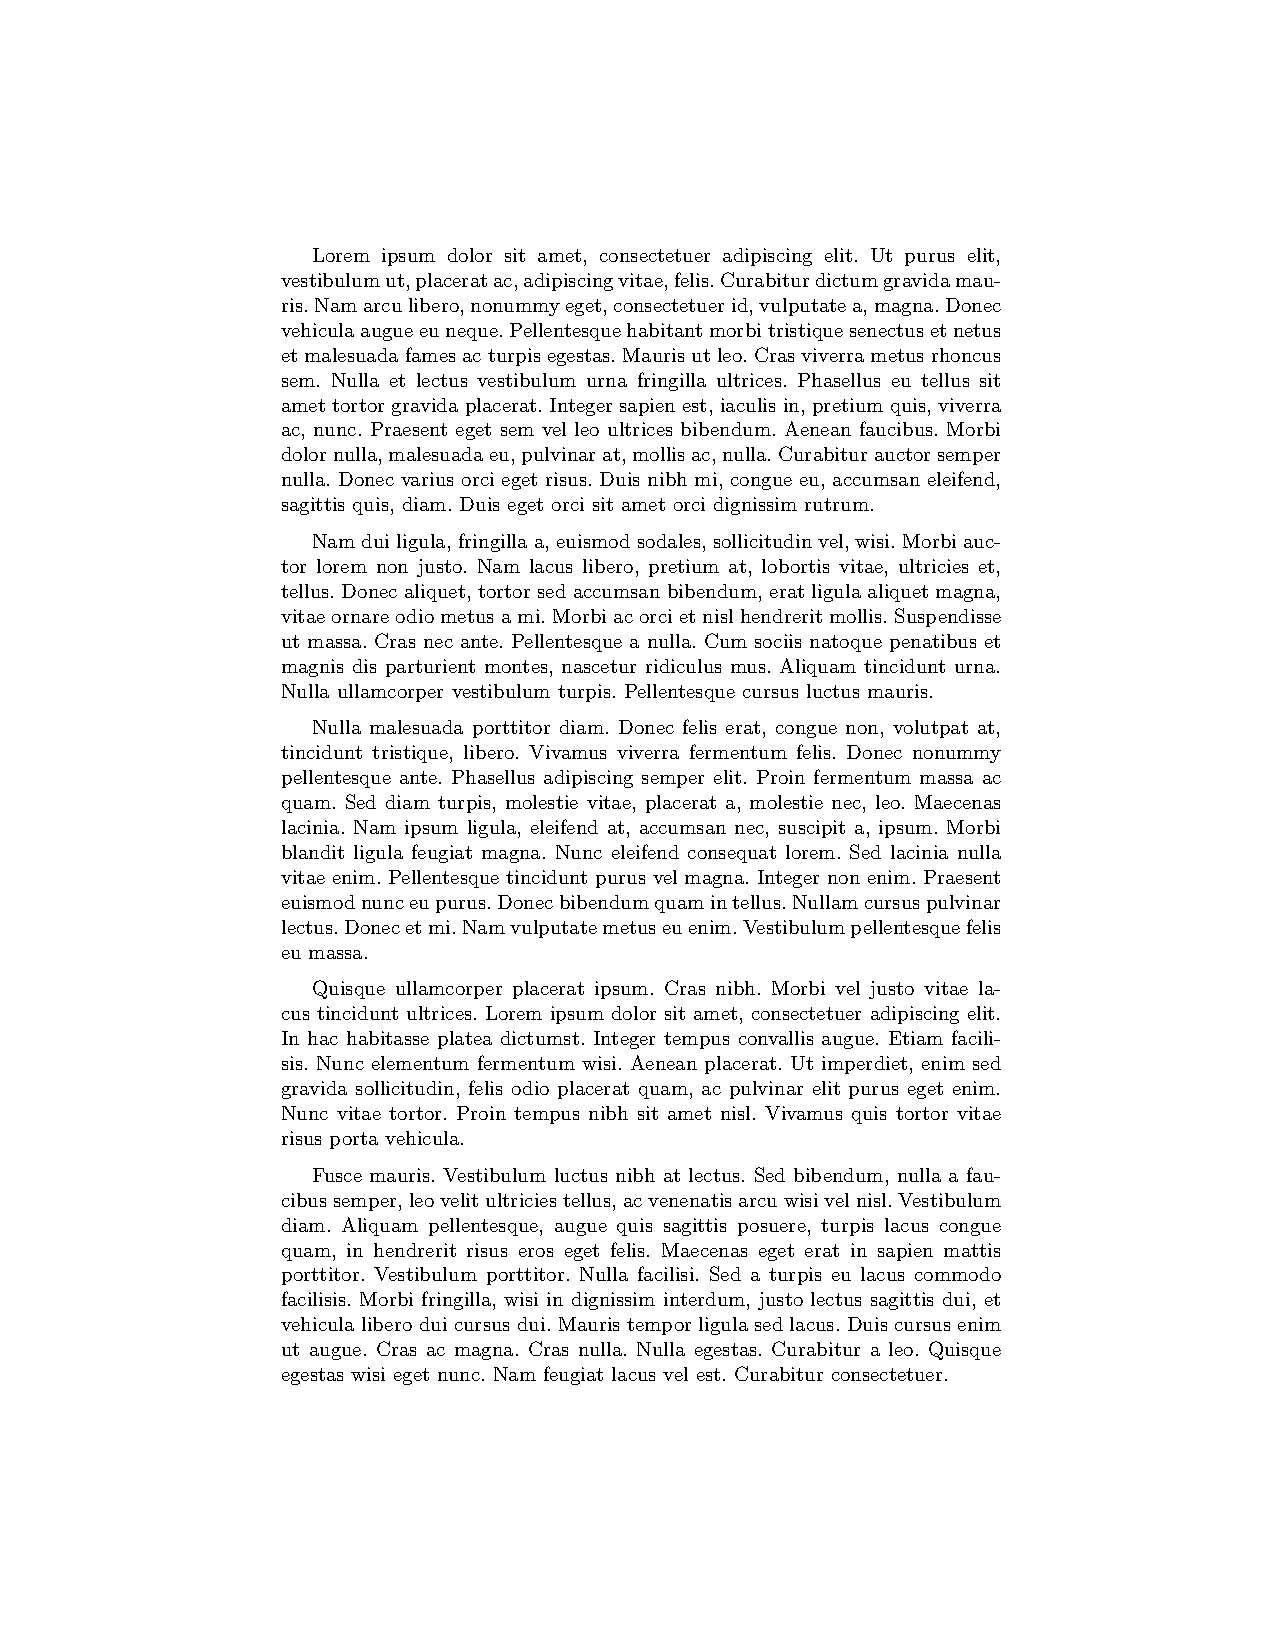
\includegraphics[page=1,width=0.412225\textwidth,trim=1.75in 1.65in 1.75in 1.5in,clip]{examples/example_7_LNCS.pdf}}%
% }%
% \strut\hfill\strut\hfill\strut%
% \subcaptionbox{Page 2 of the pdf compiled from Example~\ref{ex:llncs2}.
% }{%
% \fbox{\includegraphics[page=2,width=0.412225\textwidth,trim=1.75in 1.65in 1.75in 1.5in,clip]{examples/example_7_LNCS.pdf}}%
% }%
% \strut\hfill\strut%
% \\%
% \strut\hfill\strut%
% \subcaptionbox{Page 3 of the pdf compiled from Example~\ref{ex:llncs2}.
% }{%
% \fbox{\includegraphics[page=3,width=0.412225\textwidth,trim=1.75in 1.65in 1.75in 1.5in,clip]{examples/example_7_LNCS.pdf}}%
% }%
% \strut\hfill\strut\hfill\strut%
% \subcaptionbox{Page 4 of the pdf compiled from Example~\ref{ex:llncs2}.
% }{%
% \fbox{\includegraphics[page=4,width=0.412225\textwidth,trim=1.75in 1.65in 1.75in 1.5in,clip]{examples/example_7_LNCS.pdf}}%
% }%
% \strut\hfill\strut%
% \caption{The rendered result of Example~\ref{ex:llncs2} (with trimmed page margins): %
% A \texttt{figureSeries} floating in single-column mode (see Example~\ref{ex:llncs} for the non-floating version).}%
% \label{ex:llncs2:res}%
% \end{center}%
% \end{figure}%
%
% \afterpage{\clearpage}%
%
% \subsubsection{Mixed \texttt{figureSeries}, \texttt{figure}, and \texttt{figure*}}
% In Example~\ref{ex:mixed}, we mix |figureSeries| with |figure| and |figure*|
% environments. This would cause |Float(s) lost!| errors in version |0.9.2| of
% our package. We again use the |IEEEtran| class~\cite{IEEETRAN}.
% The result is rendered as Figure~\ref{ex:mixed:res}. As you can see, the ordering
% of the figures in the current version of our package (|0.9.4|) is far from perfect, 
% but at least the document compiles. In a productive environment, you would have more
% text between your figures, so hopefully, such layout problems would not occur.
%
% \begin{example}%
% \begin{small}\verbatiminput{examples/example_8.tex}\end{small}%
% \caption{An example for a mixture of \texttt{figureSeries}, \texttt{figure}, and \texttt{figure*}, 
% Figure~\ref{ex:mixed:res}.}%
% \label{ex:mixed}%
% \end{example}%
%
% \begin{figure}%
% \begin{center}%
% \strut\hfill\strut%
% \subcaptionbox{Page 1 of the pdf compiled from Example~\ref{ex:mixed}.
% }{%
% \fbox{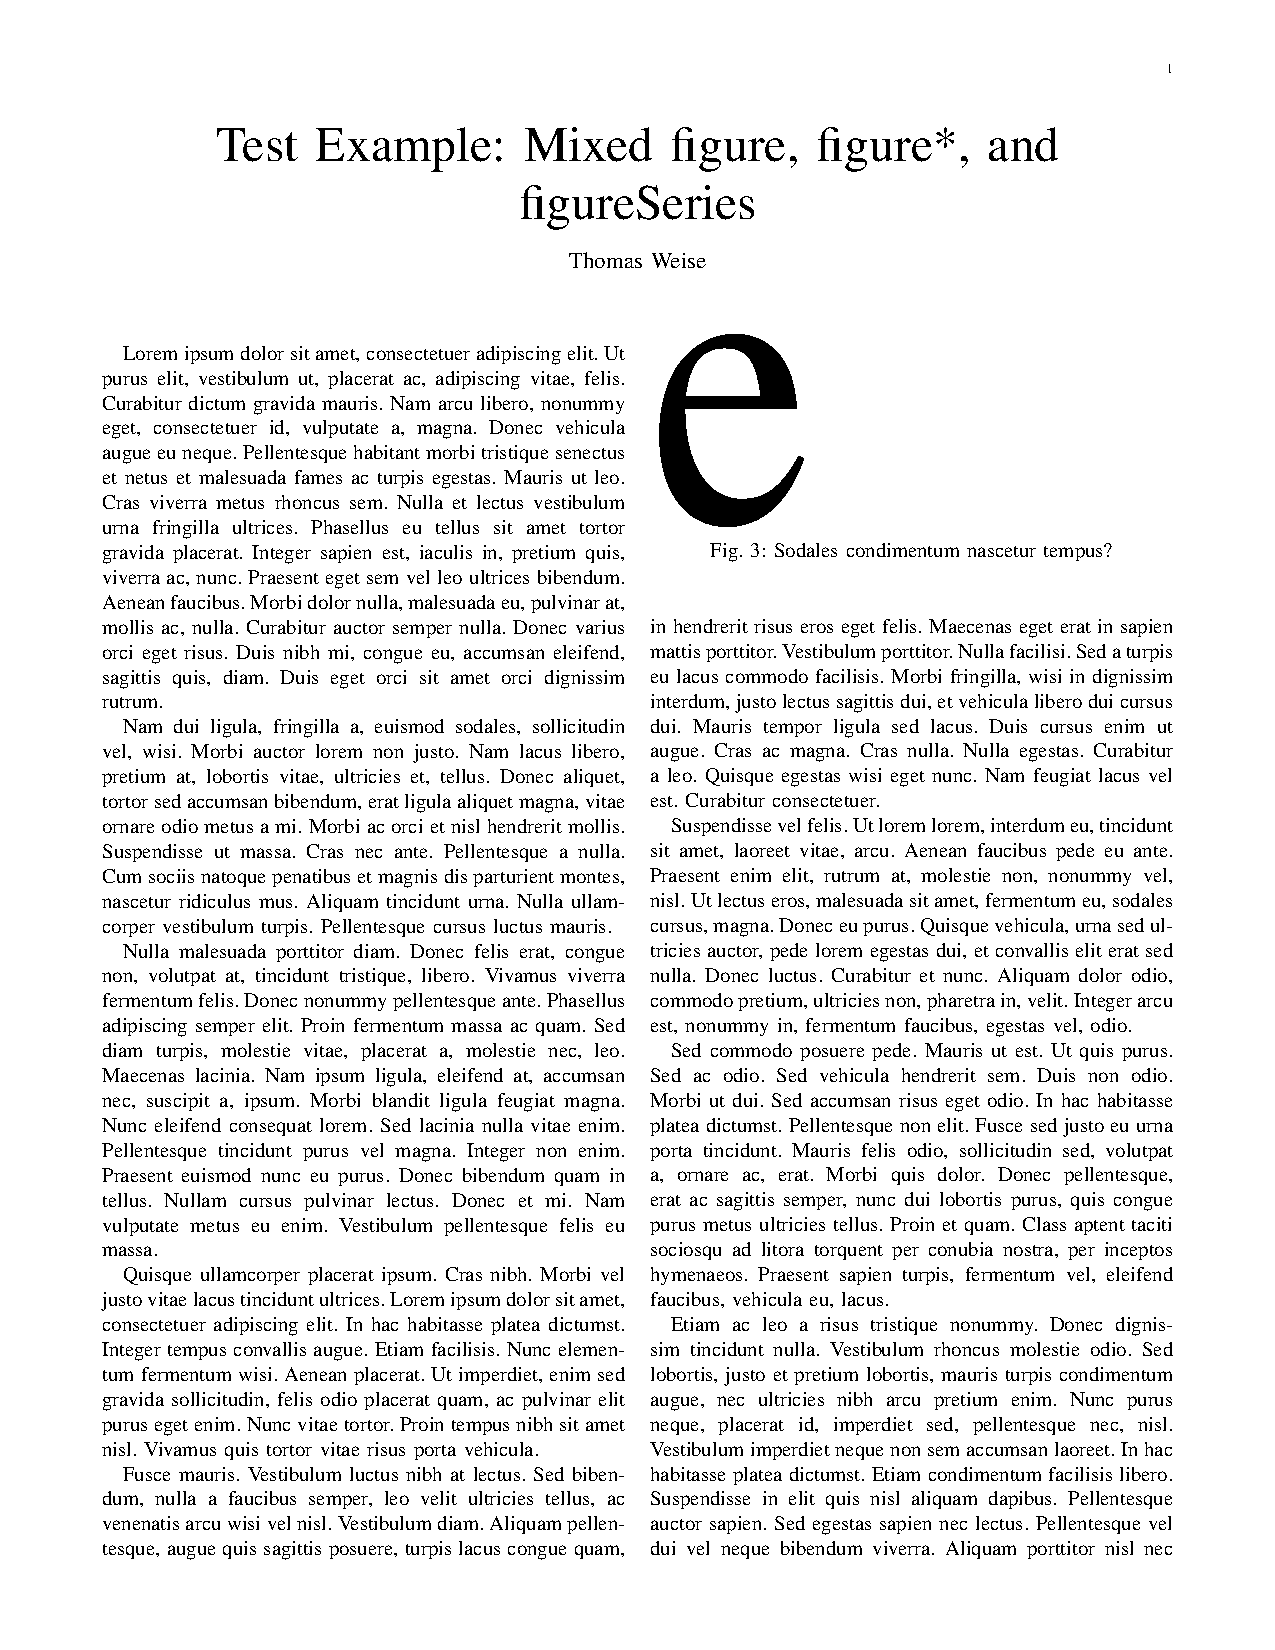
\includegraphics[page=1,width=0.45\textwidth,trim=0.65in 0.35in 0.65in 0.75in,clip]{examples/example_8.pdf}}%
% }%
% \strut\hfill\strut\hfill\strut%
% \subcaptionbox{Page 2 of the pdf compiled from Example~\ref{ex:mixed}.
% }{%
% \fbox{\includegraphics[page=2,width=0.45\textwidth,trim=0.65in 0.35in 0.65in 0.75in,clip]{examples/example_8.pdf}}%
% }%
% \strut\hfill\strut%
% \\%
% \strut\hfill\strut%
% \subcaptionbox{Page 3 of the pdf compiled from Example~\ref{ex:mixed}.
% }{%
% \fbox{\includegraphics[page=3,width=0.45\textwidth,trim=0.65in 0.35in 0.65in 0.75in,clip]{examples/example_3_IEEEtran.pdf}}%
% }%
% \strut\hfill\strut%
% \caption{The rendered result of Example~\ref{ex:mixed} (with trimmed page margins): %
% a mixture of \texttt{figureSeries}, \texttt{figure}, and \texttt{figure*}.}%
% \label{ex:mixed:res}%
% \end{center}%
% \end{figure}%
%
% \clearpage%
%
%
%
% \StopEventually{}
%
% \section{Implementation}%
%
% The names of all macros for public use are prefixed with |figureSeries|.
% The names of all internal elements of the package are prefixed with |@figSer@|.
% This naming convention should prevent any name clashes with other packages.
%
% \subsection{Loading of Required Packages}%
%
% Our |figureSeries| package requires three other packages:%
% \begin{enumerate}%
% \item The package |caption|~\cite{S2011TCPCCIFE} for the caption of the |figureSeries|.%
% \item The package |subcaption|~\cite{S2013TSPSFSC} for sub-figure layout and captions.%
% \item The package |afterpage|~\cite{C1995TAPECATPB} for creating the impression that our |figureSeries| can float.%
% \end{enumerate}%
%
% \subsubsection{Loading \texttt{caption} and \texttt{subcaption}}%
%
% We rely on the packages |caption| and |subcaption| to render the |figureSeries|'
% and sub-figure's captions. However, Springer's |llncs.cls|~\cite{SPRINGERLNCS} seems %
% to be incompatible with the |subcaption| package~\cite{S2013TSPSFSC}\footnote{According to %
% \url{http://www.michaelshell.org/tex/ieeetran/}, IEEE's |IEEEtrans.cls|~\cite{IEEETRAN}
% may also be incompatible, but it seems to works here.}.%
% Yet, we need that package for giving nice captions to the sub-figures.
% Therefore, we load the |caption| package~\cite{S2011TCPCCIFE} with option
% |compatibility=false| (which can solve this issue) if necessary.
% This is behavior governed by the Boolean flag \linebreak[3]|@figSer@captionCompatibilityFalse|, initialized to |false|.
%
%    \begin{macrocode}
\newif\if@figSer@captionCompatibilityFalse%
\@figSer@captionCompatibilityFalsefalse%
%    \end{macrocode}
%
% After the flag has been allocated and set to |false|, we check for Springer's |llncs.cls| (in a crude way).
% In case of |llncs.cls|, if we do not set the option |compatibility| of the |caption| package to |false|,
% we will get the error \emph{! Package caption Error: The `subcaption' package does not work correctly %
% in compatibility mode.}%
% 
%    \begin{macrocode}
\ifx\spnewtheorem\@undefined%
\else%
\@figSer@captionCompatibilityFalsetrue%
\fi%
%    \end{macrocode}
%
% Now we can load the |caption|~\cite{S2011TCPCCIFE} package with the right ``|compatibility|'' setting.
%
%    \begin{macrocode}
\if@figSer@captionCompatibilityFalse%
\RequirePackage[compatibility=false]{caption}%
\else%
\RequirePackage{caption}%
\fi%
%    \end{macrocode}
%
% We now load the |subcaption| package~\cite{S2013TSPSFSC} and set the caption style for sub-figures to arabic.
% The reason is that we may have many sub-figures, too many for indexes ranging only from
% \emph{a)} to \emph{z)}. By using arabic numbers, we are on the safe side.
%
%    \begin{macrocode}
\RequirePackage{subcaption}%
\DeclareCaptionSubType*[arabic]{figure}%
%    \end{macrocode}
%
% \subsubsection{Loading the \texttt{afterpage} Package}%
%
% Floating objects cannot break across pages, so we cannot really make our figure series
% float. However, by using the afterpage package, we can make it look as if
% it was floating by rendering it on the next page.
%
%    \begin{macrocode}
\RequirePackage{afterpage}%
%    \end{macrocode}
%
%
% \subsection{User Interface Macros}\label{sec:userInterfaceMacros}%
% This section contains the macros which the package user can/should access, i.e., those
% macros which have been shortly discussed in Section~\ref{sec:providedMacros}.%
% \begin{macro}{\figureSeriesElement}
% The  macro |\figureSeriesElement|\marg{caption}\marg{contents} inserts an element of the figure series, i.e., one sub-figure.
% Its first argument is the caption of the element. This argument also may contain a |\label|.
% The second argument is the graphic to print. It could, e.g., be a call to |\includegraphic|
% from the |graphicx| package~\cite{CR2014PITGB}.
%
% Spacing between sub-figures is handled dynamically via |\hfill|.
% We make sure to tell the |subcaption| that the sub-figures are sub-figures by
% setting |@captype| appropriately.
%    \begin{macrocode}
\long\gdef\figureSeriesElement#1#2{%
\strut\hfill\strut%
\edef\@captype{figure}%
\subcaptionbox{#1}{#2}%
\strut\hfill\strut%%
}%
%    \end{macrocode}
% \end{macro}
%
% \begin{macro}{\figureSeriesRow}\phantomsection\label{sec:figureSeriesRow}
% |\figureSeriesRow|\marg{contents} inserts a new row of elements (sub-figures) into
% the figure series. Its single argument should thus contain a sequence of |\figureSeriesElement|s.
% Since sub-figures are placed row-by-row, no sub-figure can span multiple rows.
%
% If the overall caption of the figure series has not yet been printed, it would be stored in
% |\@figSer@delayedCaption|. Thus, if |\@figSer@delayedCaption| is not empty,
% this macro first prints the delayed caption and then the contents of the row together in
% a |\parbox| command which is wrapped into a |center| environment. 
% The reason why we need to delay caption printing is that \LaTeX's page breaking algorithm may
% separate the caption from the first figure row if the figure series starts close to the bottom
% of the page. Thus, we pack the delayed caption together with the first row of figures into a
% |\parbox| command. |\parbox|es are not affected by page breaking and always remain as solid
% objects. If the caption has already been printed, i.e., |\@figSer@delayedCaption| is empty,
% we do not need the awkward |\parbox|.
%
% Plain |\parbox|es, however, seem to not work we with the breaking of the |figureSeries| into
% multiple pieces to facilitate page breaking later on. Thus, we need to wrap everything into
% a |center| environment. Since I am not sure why this is (see Section~\ref{sec:codeBasedOnLong2}), this may be
% one of dodgy parts of this package.
%
%    \begin{macrocode}
\long\gdef\figureSeriesRow#1{%
\begin{center}%
\ifx\@figSer@delayedCaption\@empty%
\vspace\abovecaptionskip%
\strut#1\strut%
\else%
\parbox[b]{\textwidth}{%
\@figSer@delayedCaption%
\xdef\@figSer@delayedCaption{}%
\vspace\abovecaptionskip%
\strut#1\strut%
}%
\fi%
\end{center}%
}%
%    \end{macrocode}
% \end{macro}
%
% 
% The following two macros, |\figureSeriesHere| and |\figureSeriesFloat|, basically act as switches
% according to the different situations given in Section~\ref{sec:cases}. Basically, different
% things need to be done for%
% \begin{enumerate}%
% \item the non-floating (``Here'') or floating (``Float'') case, as well as for%
% \item single-column or double-column documents.%
% \end{enumerate}%
%
% \begin{macro}{\figureSeriesHere}
% The  macro |\figureSeriesHere|\marg{caption}\marg{contents} tries to insert a non-floating figure
% series at the current position in the document. This means that it may begin wherever, well, it
% is defined, e.g., in the middle of the page.
%
% The macro has two mandatory parameters, the caption and the contents. The caption will (different from
% usual |figure|s) be put at the beginning of the figure series. The reason is that a figure series
% may span over multiple pages and having the caption at the end may be awkward. The caption text
% may contain a |\label|.
%
% The contents of a figure series should be a sequence of |\figureSeriesRow| calls.
%
% Since figure series are page-wide elements, starting them in the middle of the page only works
% in single-column documents. In two-column documents, any figure series will behave as specified in
% macro |\figureSeriesFloat| below.
%    \begin{macrocode}
\long\def\figureSeriesHere#1#2{%
\@figSer@detectColumns%
\if@figSer@isTwoColumns%
\@figSer@hereTwoCol{#1}{#2}%
\else%
\@figSer@hereOneCol{#1}{#2}%
\fi%
}%
%    \end{macrocode}
% \end{macro}
%
% \begin{macro}{\figureSeriesFloat}
% The  macro |\figureSeriesFloat|\marg{caption}\marg{contents} takes the same parameters
% as |\figureSeriesHere|, but has a float-like behavior. By using the |\afterpage| command from the
% |afterpage| package~\cite{C1995TAPECATPB}, we let it start at the following page. This is different from \LaTeX'
% normal floating behavior, but as good as we can get with page-breaking objects, I think.
%    \begin{macrocode}
\long\gdef\figureSeriesFloat#1#2{%
\@figSer@detectColumns%
\if@figSer@isTwoColumns%
\@figSer@floatTwoCol{#1}{#2}%
\else%
\@figSer@floatOneCol{#1}{#2}%
\fi%
}%
%    \end{macrocode}
% \end{macro}
%
% \subsection{Internal Utility Definitions and Macros}%
% The way in which we can create figure series in double-column mode is
% different (and very significantly more complex and dodgy) from how it works in
% single-column mode. We thus need to detect in which mode we are. This
% is done in the following code. Since my knowledge of \LaTeX\ and \TeX\
% is very limited, this may be quite a crude approach. Also, this
% code will probably not work if you load the |multicol| package.
% It will definitely not work with more than two columns.
%
% \subsubsection{Two-Column Mode Detection}
% Anyway, I first define a new Boolean flag |\if@figSer@isTwoColumns|, which will
% denote whether or not we are in two-column mode. It is initialized to |false|.
%    \begin{macrocode}
\newif\if@figSer@isTwoColumns%
\@figSer@isTwoColumnsfalse%%
%    \end{macrocode}
%
% \begin{macro}{\@figSer@detectColumns}
% The internal macro |\@figSer@detectColumns| detects whether or not
% we are in two-column mode. It will set |\if@figSer@isTwoColumns| to
% |\@figSer@isTwoColumnstrue| if yes and to
% |\@figSer@isTwoColumnsfalse| otherwise.
%    \begin{macrocode}
\def\@figSer@detectColumns{%
\@figSer@isTwoColumnsfalse%
\ifx\multicols\@undefined%
\else%
\ifnum\col@number>\@ne%
\@figSer@isTwoColumnstrue%
\fi%
\fi%
\if@twocolumn%
\@figSer@isTwoColumnstrue%
\fi%
}%
%    \end{macrocode}
% \end{macro}
%
% \subsubsection{The Four Cases}%
% \label{sec:cases}%
% Our figure series are basically nothing else than simple array of rows.
% Each |\figureSeriesRow| is a |\parbox| wrapped into a |center| environment and the
% |\figureSeriesElement|s are horizontally distributed inside using |\strut|s and |\hfill|s.
%
% There are four situations that need to be distinguished when building a |figureSeries| and
% for each of which we define an appropriate internal macro:%
%
% \begin{enumerate}%
% \item Single-column mode and |\figureSeriesHere|. This is the easiest situation,
%       we just apply the approach discussed above as-is. It will perfectly line into
%       the existing text.%
% \item Single-column mode and |\figureSeriesFloat|. In this case, we just put our
%       macro into an |\afterpage| call.
% \item Double-column mode and |\figureSeriesFloat|: This is the tricky part. We need to
%       leave double-column mode to single-column mode, insert our environment, and revert
%       back to double-column mode. This causes all sorts of problems and oddities, as discussed later.
% \item Double-column mode and |\figureSeriesHere|: Same as Double-column mode and |\figureSeriesFloat|.%
%\end{enumerate}%
%
% Anyway, before getting down to business, we first declare |\@figSer@delayedCaption| as the initially
% empty container for captions, as discussed when introducing the |\figureSeriesRow| macro in
% Section~\ref{sec:figureSeriesRow}.
%    \begin{macrocode}
\edef\@figSer@delayedCaption{}%
%    \end{macrocode}
%
% \subsubsection{Single-Column Mode}%
% Here we discuss the first two cases from Section~\ref{sec:cases}.
% \begin{macro}{\@figSer@hereOneCol}
% The internal macro performing the work of |\figureSeriesHere| in single-column mode.
% It takes the same arguments as |\figureSeriesHere|.
%    \begin{macrocode}
\long\def\@figSer@hereOneCol#1#2{%
%    \end{macrocode}
% We first store the caption in |\@figSer@delayedCaption| to later be picked up
% and printed by |\figureSeriesRow| (as discussed in Section~\ref{sec:figureSeriesRow})
% in order to prevent \LaTeX\ from putting it alone on the foot of a page.%
% We put the caption into a separate |\parbox|,
% because otherwise the first row of sub-figures will have captions on top instead of
% below (for some reason not clear to me).
%    \begin{macrocode}
\def\@figSer@delayedCaption{%
\noindent\parbox{\textwidth}{%
\captionof{figure}{#1}%
%    \end{macrocode}
% This command makes the figure caption counter's value global, preserving it
% for outside the |\parbox|. Otherwise, the figure counter would always remain 0
% (if only |figureSeries| are used).
%    \begin{macrocode}
\global\advance\c@figure by 0%
}%
\par}%
%    \end{macrocode}
% Put the contents of the figure series.
%    \begin{macrocode}
\begin{center}%
#2%
\end{center}%
%    \end{macrocode}
% After the figure series body, we add some small spacing to prevent the text from
% starting too close to it.
%    \begin{macrocode}
\medskip%
}%
%    \end{macrocode}
% \end{macro}
%
% \begin{macro}{\@figSer@floatOneCol}
% The internal macro performing the work of |\figureSeriesFloat| in single-column mode.
% It takes the same arguments as |\figureSeriesFloat|.
% It basically places the output created by |\@figSer@hereOneCol| into an |\afterpage| call,
% giving it the same look-and-feel as |\@figSer@hereOneCol| while also looking like a
% floating object.
%    \begin{macrocode}
\long\def\@figSer@floatOneCol#1#2{%
\afterpage{\@figSer@hereOneCol{#1}{#2}}%
}%
%    \end{macrocode}
% \end{macro}
% 
% \subsubsection{Double-Column Mode}%
% \label{sec:doubleColumn}%
% Here we discuss the last two cases from Section~\ref{sec:cases}.
%
% Documents with two columns create a big headache. After a long search, I think I have
% more or less got a working solution. The problem is as follows:%
%
% \paragraph{A.}%
% Figure series make only sense as page-wide constructs. Figure series can include a sequence
% of many figures which may span over multiple pages. If we would restrict them to single-column
% elements, then they could start in the middle of left column and end in the middle of the
% right column. That would look very odd. Also, it is our goal to create something which looks
% more or less the same, regardless whether the document is typeset as single- or double-column.%
%
% \paragraph{B.}\phantomsection\label{sec:doubleColumnToSingleColumn}%
% This means we need to switch to single-column mode if we are in double-column mode. We can
% do that with the |\onecolumn| command, but this will always begin a new page. This
% could mean that we get a (true) page break after only half of the left column. This would
% look odd. But OK, we can define figure series in double-column mode as floating objects
% by default and use the same |\afterpage| facility that we used to make figure series in
% single-column mode float. We then just put the |\onecolumn| into the stuff we float away
% with |\afterpage| and avoid the ugly page break in the middle of the text.
%
% \paragraph{C.}%
% In double-column mode, |\afterpage| behaves more like ``|\aftercolumn|''. That is, if we
% are currently in the left column, its contents will not be rendered at the start of the
% next page, but at the start of the right column. Only if we are in the right column,
% it will put our stuff on the next page. Well, this is already the answer: If we are
% in the left column, we do something like |\afterpage{\afterpage{...}}|.%
%
% \paragraph{D.}\phantomsection\label{sec:switchToTwoColumn}%
% The biggest problem is that we need to switch back to double-column mode after our
% figure series. We can do that with the |\twocolumn| command, but this will entail
% a |\clearpage| afterwards. This means that even if our figure series only occupies the top
% 20\% of a page, there will be a page break, leaving the rest of the page blank before
% continuing in double-column mode.%
%
% \paragraph{E.}\phantomsection\label{sec:long2}%%
% After searching for a long time for a solution, I found a lead in an answer to the
% StackOverflow question \url{http://tex.stackexchange.com/questions/74433} on a vaguely
% reated issue. In his answer~\cite{H2012MPOCAIATCD}, Tom{\'{a}}{\v{s}}~Hejda introduced
% a way to switch to the |\twocolumn| mode and prepending a long series of vertical
% boxes. I simply copied his code from the answer into this package but renamed all
% involved entities to fit to our internal naming scheme.
%
% \paragraph{F.}\phantomsection\label{sec:extendBody}%
% Still, there is another problem: If more than one figure series is started on
% the same page, then we may get an empty page inbetween because of the |\clearpage|
% done by |\onecolumn|. The trick here is to detect whether another figure series
% is ``scheduled'' but not yet laid out. In this case, we attach the contents
% of our new figure series to the contents of the pending one (stored in a body macro)
% via |\g@addto@macro|. After the figure series is actually laid out, the body macro
% must be emptied.
%
% \paragraph{G.}\phantomsection\label{sec:floatsLost}%
% The final problem we need to deal with is the fact that |afterpage|~\cite{C1995TAPECATPB}
% has neither been designed for two-column documents nor for situations with other
% floats flying around. This may lead to  |Float(s) lost!| errors. My first attempt (in version |0.9.3|) to
% solve this was by issuing a |\FloatBarrier| (from package |placeins|~\cite{A2005TPP})
% in an |\AddThispageHook| from package |everypage|~\cite{C2007TEP}. This makes the error
% disappear in some documents (such as in Example~\ref{ex:mixed}), but it re-appears in
% other documents, which previously compiled well.
% 
% Alltogether, this is a bit of a Frankenstein's monster. Anyway, here we go with the code.
%
% Let us first allocate a macro placeholder |\@figSer@floatingBody| for the floating figure series body
% (see \mbox{Section~\ref{sec:extendBody}.G}),
% which will later be filled in by |\@figSer@hereTwoCol|.
%    \begin{macrocode}
\xdef\@figSer@floatingBody{}%
%    \end{macrocode}%
%
%
% \begin{macro}{\@figSer@floatTwoCol}
% The internal macro performing the work of |\figureSeriesFloat| in two-column mode.
%    \begin{macrocode}
\long\def\@figSer@floatTwoCol#1#2{%
%    \end{macrocode}
% If no figure series is pending, we build the figure series ``body'' exactly as in
% the single-column case, but instead of laying it out directly, it is stored in the
% |\@figSer@floatingBody| macro.
%    \begin{macrocode}
\ifx\@figSer@floatingBody\@empty%
\gdef\@figSer@floatingBody{\@figSer@hereOneCol{#1}{#2}}%
%    \end{macrocode}
% Ok, we have now created the body of our figure series, but it is not yet ``floating''.
% We let it float by putting it into an |\afterpage| if we already are in the
% second (right) column (|\if@firstcolumn| is false) or into two nested |\afterpage|s, if we
% are in the first (left) column (|\if@firstcolumn| is true).
%    \begin{macrocode}
\if@firstcolumn%
\afterpage{\afterpage{\@figSer@twoColPrintBody}}%
\else%
\afterpage{\@figSer@twoColPrintBody}%
\fi%
%    \end{macrocode}
% End of ``new'' figure series.
%    \begin{macrocode}
\else%
%    \end{macrocode}
% OK, if we get here, a figure series is pending. In this case, the body of the current
% figure is appended to it as discussed in \mbox{Section~\ref{sec:extendBody}.G}. We do not need
% to |\afterpage| a call to |\@figSer@twoColPrintBody| since there must already be one enqueued.
%    \begin{macrocode}
\g@addto@macro{\@figSer@floatingBody}{\@figSer@hereOneCol{#1}{#2}}%
\fi%
}%
%    \end{macrocode}
% \end{macro}
%
% \begin{macro}{\@figSer@hereTwoCol}
% The macro |\@figSer@hereTwoCol| represents the fourth case listed in Section~\ref{sec:cases}.
% Since there is no way we can have a page-wide object in the middle of a double-column page
% that I know of, for now, this case simply behaves like the double-column floating case.
%    \begin{macrocode}
\let\@figSer@hereTwoCol\@figSer@floatTwoCol%
%    \end{macrocode}
% \end{macro}
%
% \subsubsection{Switch back to \texttt{twocolumn} According to~\cite{H2012MPOCAIATCD}}%
% \label{sec:codeBasedOnLong2}%
% Here I include the code provided by Tom{\'{a}}{\v{s}}~Hejda in his answer to
% question \url{http://tex.stackexchange.com/questions/74433}~\cite{H2012MPOCAIATCD}.
% Instead of copy-pasting it, I changed all naming to match this package's convention and
% made one minor modification. The name changing has two reasons: First, it ensures that
% all parts of this package follow the same naming convention and can easily be identified
% as parts of this package. Second, if Tom{\'{a}}{\v{s}}~Hejda should turn his code into
% a package (as his answer~\cite{H2012MPOCAIATCD} indicated), there will be no name clashs
% between his package and mine.
%
% \emph{I must point out that I do not really understand this code. I understand roughly
% what it does, but there are several nuances which are unclear to me.}
%
% Also, some of the numbers, like for the page height fraction (0.84) or the
% |vspace| (15pt plus 15pt), seem to be fixed to somewhat arbitrary values, which may
% be better taken from the current configuration (like |\floatpagefraction| or
% |\medskip| something). Right now, I don't have the nerve to check for this,
% but I may check this again in the future.
%
% Furthermore, I don't understand much about \LaTeX\ box registers, which is
% maybe why I find it a bit dangerous to use boxes at low indexes (|0|, |1|, |2|).
% Maybe some box registers should explicitly be allocated in one way or another?
% I am not sre. This probably really is correct, but as I have too limited knowledge, 
%
% Anyway, let's begin with the code. First, a new |newsavebox| is allocated.
%    \begin{macrocode}
\newsavebox\@figSer@box%
%    \end{macrocode}
%
% This macro is represents the body of the figure series. In a loop, chunks
% as big as possible but small enough to fit on a page are cut off and printed.
% Different from~\cite{H2012MPOCAIATCD}, we implement this macro for re-use
% in the next figure series. The equivalent |\longtwo@repeat| macro in~\cite{H2012MPOCAIATCD}
% seems to ultimately overwritten and, from what I can see at first glance
% without testing, can only be used once.
%  \begin{macro}{\@figSer@breakBodyRepeat@Orig}
%    \begin{macrocode}
\def\@figSer@breakBodyRepeat@Orig{%
%    \end{macrocode}
% We first switch from two-column to single-column mode (|\@twocolumnfalse|).
% Then, the elements of the figure series' are printed on top of the page
% spanning both columns (since the code for that is the parameter to |\twocolumn|).
% Finally, |\twocolumn| switches to two-column mode. 
%    \begin{macrocode}
\twocolumn[{\@twocolumnfalse%
%    \end{macrocode}
% Once and only once, we store the contents of |\@figSer@floatingBody| into the box
% |\@figSer@box|. Once this is done, |\@figSer@floatingBody| is set to |\@empty|. 
%    \begin{macrocode}
\ifx\@figSer@floatingBody\@empty%
\else%
\global\setbox\@figSer@box\vbox{\@figSer@floatingBody}%
\global\let\@figSer@floatingBody\@empty%
\fi%
%    \end{macrocode}
% Check if the contents of our box fit on the current page. 
%    \begin{macrocode}
\ifdim\ht\@figSer@box>\textheight%
%    \end{macrocode}
% If the contents of our box are bigger then the |\textheight|, we split
% the box and output the first part on the current page.
%    \begin{macrocode}
\begingroup%
\vbadness10000%
\setbox0\vsplit\@figSer@box to \textheight%
\setbox1\vbox{\unvbox\@figSer@box}%
\global\setbox\@figSer@box\vbox{\unvbox1}%
\setbox2\vbox to \textheight{%
\unvbox0%
}%
\ht2=0.9\textheight%
\box2%
\endgroup%
\else%
%    \end{macrocode}
% If the contents of our box fit on the page but are large, we will issue a |\clearpage|
% after printing them, otherwise we print them and do nothing.%
%    \begin{macrocode}
\ifdim\ht\@figSer@box>0.84\textheight%
\global\let\@figSer@breakBodyRepeat\clearpage%
\else%
\global\let\@figSer@breakBodyRepeat\relax%
\fi%
\unvbox\@figSer@box%
\vspace{15pt plus 15pt}%
\fi%
}]%
%    \end{macrocode}
% We use recursion to iterate the body loop.
%    \begin{macrocode}
\@figSer@breakBodyRepeat%
}%
%    \end{macrocode}
%  \end{macro}%
%
%  \begin{macro}{\@figSer@twoColPrintBody}
% This is the main entry point to our version of Tom{\'{a}}{\v{s}}~Hejda's method~\cite{H2012MPOCAIATCD},
% equivalent to his |\longtwo@| macro, with the slight difference that we restore |\@figSer@breakBodyRepeat|
% and thus can use this macro multiple times.
%    \begin{macrocode}
\long\def\@figSer@twoColPrintBody{%
\let\@figSer@breakBodyRepeat\@figSer@breakBodyRepeat@Orig%
\begingroup%
\@figSer@breakBodyRepeat%
\endgroup%
}%
%    \end{macrocode}
%  \end{macro}
%
% \subsection{Tests and Incompatibilities}%
% \label{sec:incompatible}%
%
% |figureSeries| loads the packages |caption|~\cite{S2011TCPCCIFE},
% |subcaption|~\cite{S2013TSPSFSC}, and |afterpage|~\cite{C1995TAPECATPB}.
% Therefore it inherits all incompatibilities of these packages. The |subcaption| package, for instance,
% is not compatible with the packages |subfigure| and |subfig|.
%
% \subsection{Related Work}%
% The |longfigure| package~\cite{A2014TLPPAFLETBOP} provides a similar functionality,
% i.e., a figure environment that can wrap over multiple pages. This environment can
% be made to float by using |\afterpage|, but does not work in double-column documents.
%
% Tom{\'{a}}{\v{s}}~Hejda's method~\cite{H2012MPOCAIATCD}, which is used by our
% package, may be extended to provide similar functionality, if it is published
% as package as indicated in~\cite{H2012MPOCAIATCD}.
%
% \subsection{License}%
% The copyright (c) of this work is with Thomas Weise (\url{http://www.it-weise.de})
% except for the code in Section~\ref{sec:codeBasedOnLong2}. The code
% in Section~\ref{sec:codeBasedOnLong2} is a modified version from
% Tom{\'{a}}{\v{s}} Hejda's (\href{mailto:tohecz@gmail.com}{tohecz@gmail.com}) answer~\cite{H2012MPOCAIATCD} to
% question \url{http://tex.stackexchange.com/questions/74433}. The copyright of this
% is thus not clear to me, so I won't claim it :-)
%
% This document, the package, and its documentation are under the LaTeX Project Public License, version 1.3,
% which may be found online at \url{http://www.latex-project.org/lppl.txt}.
% 
% The distribution of this package may also contain the \LaTeX\ document classes
% |llncs.cls|~\cite{SPRINGERLNCS}, |IEEEtran.cls|~\cite{IEEETRAN}, and |sig-alternate.cls|~\cite{ACMSIGALTERNATE}.
% The copyrights of these files are with their respective owners and these owners
% alone can determine the license terms for these files. The files are just
% included here to make the examples stand-alone. They may not be up-to-date,
% so please download their latest versions from their respective locations.
%
% If you feel that this document, its presentation, or any parts I provide for
% download violate your (copy)right, please contact me (\url{http://www.it-weise.de},
% \href{mailto:tweise@ustc.edu.cn}{tweise@ustc.edu.cn}, \href{mailto:tweise@gmx.de}{tweise@gmx.de})
% and I will immediately resolve the issues.
%
% 
% \begin{thebibliography}{10}
% \providecommand{\natexlab}[1]{#1}
% \providecommand{\url}[1]{\texttt{#1}}
% \expandafter\ifx\csname urlstyle\endcsname\relax
%   \providecommand{\doi}[1]{doi: #1}\else
%   \providecommand{\doi}{doi: \begingroup \urlstyle{rm}\Url}\fi
% 
% \bibitem[Weise et~al.(2014)Weise, Chiong, Tang, L{\"{a}}ssig, Tsutsui, Chen,
%   Michalewicz, and Yao]{WCTLTCMY2014BOAAOSFFTTSP}
% Thomas Weise, Raymond Chiong, Ke~Tang, J{\"{o}}rg L{\"{a}}ssig, Shigeyoshi
%   Tsutsui, Wenxiang Chen, Zbigniew Michalewicz, and Xin Yao.
% \newblock {Benchmarking Optimization Algorithms: An Open Source Framework for
%   the Traveling Salesman Problem}.
% \newblock \emph{IEEE Computational Intelligence Magazine (CIM)}, 9\penalty0
%   (3), August 2014. \doi{10.1109/MCI.2014.2326101}, \url{http://www.it-weise.de/documents/files/WCTLTCMY2014BOAAOSFFTTSP.pdf}
% 
% \bibitem[Kushwah(2009)]{K2009SOAFOMP}
% Hemant~Ritturaj Kushwah.
% \newblock {Subfigs of a Figure on Multiple Pages}, July 3, 2009.
% \newblock URL \url{http://stackoverflow.com/questions/1078370}.
% 
% \bibitem[arjmage and Vogt(2011)]{AV2011SSAMPBP}
% arjmage and Hendrik Vogt.
% \newblock {Splitting subfigures across multiple pages {--} but
%   programmatically!}, February~14, 2011.
% \newblock URL \url{http://tex.stackexchange.com/questions/11059}.
% 
% \bibitem[Munch(2012)]{MH2012TMP}
% Hanns-Martin M{\"u}nch and Don Hosec
% \newblock \emph{The morefloats Package}, January~28, 2012, version v1.0f
% \newblock URL \url{http://www.ctan.org/pkg/morefloats}
%
% \bibitem[Sommerfeldt(2011)]{S2011TCPCCIFE}
% Axel Sommerfeldt.
% \newblock \emph{{The caption Package {--} Customising captions in floating
%   environments}}, November~2, 2011.
% \newblock URL \url{http://www.ctan.org/pkg/caption}.
% 
% \bibitem[Sommerfeldt(2013)]{S2013TSPSFSC}
% Axel Sommerfeldt.
% \newblock \emph{{The subcaption package {--} Support for sub-captions}}, April~16, 2013.
% \newblock URL \url{http://www.ctan.org/pkg/subcaption}.
% 
% \bibitem[Carlisle(1995)]{C1995TAPECATPB}
% David P.\ Carlisle.
% \newblock \emph{{The afterpage Package {--} Execute command after the next page
%   break}}, October~27, 1995.
% \newblock URL \url{http://www.ctan.org/pkg/afterpage}.
%
% \bibitem[Carlisle(2014)]{CR2014PITGB}%
%  David P.\ Carlisle and Se­bas­tian Rahtz.%
% \newblock \emph{Packages in the `graphics' bundle}, April~27, 2014.%
% \newblock URL \url{http://www.ctan.org/pkg/graphicx}.%
%
% \bibitem[Happel(2014)]{H2914LAT1POLIDT}
% Patrick Happel.%
% \newblock \emph{lipsum -- Access to 150 paragraphs of Lorem ipsum dummy text},%
% July~27, 2014.
% \newblock URL \url{http://www.ctan.org/pkg/lipsum}.%
% 
% \bibitem[SPR(2010)]{SPRINGERLNCS}
% {LLNCS Document Class {--} Springer Verlag LaTeX2e support for Lecture Notes in
%   Computer Science}, June 12, 2010.
% \newblock URL
%   \url{ftp://ftp.springer.de/pub/tex/latex/llncs/latex2e/llncs2e.zip}.
% 
% \bibitem[Murray et~al.(2007)Murray, Balemi, Dixon, N{\"{u}}chter, {von Hagen},
%   and Shell]{IEEETRAN}
% Gerald Murray, Silvano Balemi, Jon Dixon, Peter N{\"{u}}chter, J{\"{u}}rgen
%   {von Hagen}, and Michael Shell.
% \newblock {Official IEEE LaTeX Class for Authors of the Institute of Electrical
%   and Electronics Engineers (IEEE) Transactions Journals and Conferences}, May~3, 2007.%
% \newblock URL \url{http://www.michaelshell.org/tex/ieeetran/}.%
% 
% \bibitem[Murray and Tobin(2009)]{ACMSIGALTERNATE}
% Gerald Murray and G.K.M. Tobin.
% \newblock {SIG-ALTERNATE.CLS {--} Version 2.4 (Compatible with the%
%   ACM{\_}PROC{\_}ARTICLE-SP.CLS`` V3.2SP)}, April~22, 2009.%
% \newblock URL \url{http://www.acm.org/sigs/publications/proceedings-templates}.%
%
% \bibitem[Callegari(2007)]{C2007TEP}
% Sergio Callegari.
% \newblock \emph{{The Everypage Package}}, June~20, 2007.
% \newblock URL \url{http://www.ctan.org/pkg/everypage}%
%
% \bibitem[Arseneau(2005)]{A2005TPP}
% Donald Arseneau.
% \newblock \emph{The Placeins Package}, April~18, 2005.
% \newblock URL \url{http://www.ctan.org/pkg/placeins}
% 
% \bibitem[Arnold(2014)]{A2014TLPPAFLETBOP}
% Tim Arnold.
% \newblock \emph{{The longfigure Package {--} Provides a figure-like environment%
%   that break over pages}}, January~6, 2014.%
% \newblock URL \url{http://www.ctan.org/pkg/longfigure}.%
%
% \bibitem[Hejda(2012)]{H2012MPOCAIATCD}%
% Tom{\'{a}}{\v{s}} Hejda (answer, email: \href{mailto:tohecz@gmail.com}{tohecz@gmail.com}), Augustin (question)%
% \newblock \emph{Multi-Page One-Column Abstract in a Two-Column Document}, %
% September~27, 2012.%
% \newblock URL \url{http://tex.stackexchange.com/questions/74433}.%
% 
% \end{thebibliography}
% \Finale
\endinput
